\documentclass[review]{elsarticle}

\usepackage{lineno,hyperref}
\usepackage{rotating}
\usepackage{algpseudocode,algorithm}
\usepackage{hyperref}
\usepackage{listings}
\usepackage{xcolor}
\usepackage{multirow}
\usepackage[normalem]{ulem}
\useunder{\uline}{\ul}{}

\lstset{
basicstyle=\small\ttfamily,
}

\graphicspath{ {./images/} }

\modulolinenumbers[5]

\journal{Future Generation Computer Systems}
\begin{document}
\lstset{language=Python} 
\begin{frontmatter}

\title{EvoSwarm: A Cloud-Native Architecture for the Reproducible Execution of Multi-population Optimization Algorithms}

\author[itt]{Mario Garc\'ia Valdez}\corref{mycorrespondingauthor}
\cortext[mycorrespondingauthor]{Corresponding author}
\ead{mario@tectijuana.edu.mx}

\author[granada]{Juan J. Merelo Guerv\'os}
\ead{jmerelo@geneura.ugr.es}

\address[itt]{Department of Graduate Studies, Instituto Tecnol\'ogico de Tijuana, Tijuana BC, Mexico}
\address[granada]{Department of Computer Architecture and Technology, Universidad de Granada, Granada, Spain}

\begin{abstract} 
Splitting a population into multiple instances is a technique that has
been used extensively in recent years in order to help improve the
performance of nature-inspired optimization algorithms. Work on those
populations can be done in parallel, and they can interact asynchronously,
a fact that can be leveraged to create scalable implementations based
on, among other methods, distributed, multi-threaded, parallel, and
cloud-native computing.  However, the design of these cloud-native,
distributed, multi-population algorithms is not a trivial task. Coming
from monolithic (single-instance) solutions, adaptations at several
levels, from the algorithmic to the functional, must be made to
leverage the scalability, elasticity, (limited) fault-tolerance,
reproducibility, and cost-effectiveness of cloud systems while, at the
same time, conserving the intended functionality. Instead of an
evolutive approach, in this paper we propose to create from scratch a
cloud-native optimization framework that is able to include multiple
algorithms and use few parameters to work. This solution goes beyond
current state of the art via a framework that is able to support
different algorithms at the same time, work asynchronously, and also
be easily deployable to any cloud platform. We evaluate the
performance and scalability of this solution, together with the effect
other design parameters had on it; in particular, the number and the
size of populations with respect to problem size. The architecture and
the implemented platform is an excellent alternative for running
locally or in the cloud, thus proving that cloud-native bioinspired
algorithms perform better in their ``natural'' environment than other
kinds of algorithms, % Did we compare it to other kind of algorithms?
                     % If we didn't, this should go - JJ 
                     % Compared against GA and PSO and others from BBOB - Mario
                     % on the algorithm, not speedup 
                     % I like the sentence, If we did not prove it, 
                     % at least we build a tool that will allow
                     % algorithms to run in their natural environment.
                     % The focus of the Journal after all is in computer systems - M

and setting a new baseline for scaling and
performance in the cloud.
\end{abstract}

\begin{keyword}
Multi-population \sep Nature-inspired algorithm \sep Parallel Genetic Algorithms \sep Cloud-Computing
\sep Event-driven architecture 
\end{keyword}

\end{frontmatter}

\linenumbers

\section{Introduction}

In the last decades, nature-inspired optimization algorithms have been successfully
applied to solve many complex real-world problems
\cite{yang2014nature}; these algorithms can be broadly grouped into evolutionary algorithms (EAs)
\cite{back1996evolutionary} and swarm intelligence (SI)
\cite{kennedy2006swarm}, as well as other categories; popular EAs
are Genetic Algorithms (GAs) \cite{holland1992adaptation,eiben2003genetic}, 
Genetic Programming (GP) \cite{back1996evolutionary}, Grey Wolf Optimization
(GWO) \cite{mirjalili2014grey} and Differential Evolution (DE) \cite{karabouga2004simple},
while examples of (SI) \cite{kennedy2006swarm} are particle swarm
optimization (PSO) \cite{clerc2010particle} and ant colony algorithms (ACO) \cite{dorigo1999ant}.

Besides being all population-based, they also share the common characteristic
of creating an initial set of random candidate solutions that are later used to
generate a new set of candidates, using a nature-inspired heuristic.
Population-based algorithms are intrinsically parallel, and can be implemented to run asynchronously.
The fitness of each individual can be (in general) evaluated independently of 
others, and similarly, each population could evolve in isolation. Researchers use the term
multi-population based methods when generally referring to techniques using
many populations as part of their optimization strategy. 
Since 
earlier works, researchers have been proposing some form of parallelization
\cite{muhlenbein1988evolution} to increase the scalability of these
algorithms that adds to this simple parallel execution some form of
interaction between the independently running populations.
The island model was one of the first techniques proposed for parallelization,
which led to an early proof of speedup   \cite{gorges1990explicit,grosso1985computer}. 
The concept was to divide a large population into communicated subpopulations. 
Since then, other population-based algorithms have adopted the concept, 
and researchers have found additional benefits
besides the execution speed; these include avoiding a premature convergence and
maintaining the diversity of the global population \cite{li2015multi}. 

% Probably it's not the time for this, but maybe it would be interesting to 
% mention that asynchronous implementations in most cases need a change in 
% the underlying algorithm, while synchronous might not need it - JJ 
% TO DO - Mario 
Moreover, parallel implementations can run in two different ways: synchronous and
asynchronous. When operations run in parallel but every node must maintain synchrony with
the other operations,  all operations need to finish to continue to the next
step. For instance, in a  master/worker model, the master needs to wait for all
workers to finish their operations before moving to the next iteration.  In
contrast, in an asynchronous execution,  operations are not synchronized with
each other, so there's no time lost waiting for other populations to
arrive to the synchronization point; results arriving from other workers are 
incorporated as soon as they are received. Following the previous example, now the master operation can
continue to the next iteration, even if a worker has not finished its work.  In
the literature, we can find many asynchronous algorithms
\cite{coleman89,baugh2003asynchronous}, reporting benefits in execution time,
and scalability. In the particular case of asynchronous and cloud-native
multi-population algorithms, recent works propose an asynchronous communication
through a central repository \cite{sofea:cec2012, JSON} or message queues
\cite{salza2019speed, guervos2018introducing}, in this work we follow this
practice.

The trend concerning the parallel execution multi-population algorithms goes from
earlier hardware-based implementations using transputers
\cite{gorges1990explicit} through 
multi-core systems \cite{Serrano2008,lai2019adaptive} to multi-threaded \cite{merelo2019scaling} ones.
And recently the focus has been on exploiting a higher number of processing
units by using GPUs \cite{tan2015survey,li2007efficient}, or distributed
systems, including web-based \cite{JSON} systems,
map-reduce \cite{fazenda2012} implementations,  grids \cite{munawar2010design,Gonzalez09},
voluntary computing systems \cite{MilkyWay,merelo2016nodio}, 
and, more importantly, cloud computing
\cite{GValdez2015,salza2019speed,valenzuela2015implementing,FlexGP}. Cloud computing has become the standard way of running
enterprise applications, not only because of the convenience of the
pay-as-you-go model or the non-existent sunk cost of physical facilities, but also because
it offers a way of describing the infrastructure as part of the code, so that it
is much easier to reproduce results and this has been a boon for scientific
computing.  However,  cloud computing has also been evolving, going from simply
putting on virtual machines elsewhere than on premises old-style monolithic applications, that is, applications
built on a single stack of services that communicate by layers, to microservices
\cite{microservices} and serverless architectures \cite{varghese2018next,Varghese2018849} that favor the parallel and asynchronous communication of
heterogeneous resources; in the process, a new methodology for designing {\em cloud
native applications} has been created, with brand new methods and
techniques \cite{Baldini2016287}. In these architectures, services or even
functions are seen as independent processing nodes, departing from the monolithic
and even distributed paradigms, and becoming a loosely coupled collection of {\em
stateless functions} \cite{malawski2017serverless}, that react to events and
only come into existence while they are doing some processing.
Systems developed with the patterns outlined above have the
properties of a reactive system \cite{boner2014reactive} and they are commonly
more flexible, fault-tolerant, and scalable. % Some properties and reference - Mario  
% Again, you have to justify the need for a reactive architecture and define it before this paragraph - JJ

Researchers 
and algorithm designers willing to  adapt to the cloud their
multi-population solutions face the additional challenges:
\begin{itemize}
    \item They need to change their current solutions to a reactive architecture in which processes
    communicate with each other by exchanging messages asynchronously and react
    to a continuous stream of data. One of the options is to consider
    populations as messages to be modified asynchronously by functions. 

    \item To scale the system, when it is possible, there are several options, including the  use of stateless functions for
    processing. 

    \item They need to establish a workflow of local development and prototyping while having the 
    option of deployment in a cloud provider. It is desirable to use modern development methodologies and technologies. 

    \item They must log experimental results and be able to replicate the experiments. 

    \item They must consider additional parameters that can affect the monetary cost or the performance of the
    execution — for instance, the format and size of messages, the number of
    worker processes and their capabilities.  
\end{itemize}

% I have moved these sentences here, since they seem to fit the best.(OK - M)
Beyond the choice of design methodology and implementation, researchers need to
consider additional issues \cite{Ma2019} when designing efficient multi-population algorithms. These include the number and size of populations,
the interaction between them, the search area of each population, and the search
strategy and parametrization of each population. We must take into account
these high-level issues when designing a parallel architecture.

Taking these factors into account, in this work, we present EvoSwarm, 
a container-based application that reactively processes
isolated and
heterogeneous populations. The platform uses the {\tt docker-compose} tool for
defining and running experiments as multi-container applications. EvoSwarm is also released with a free licence in \url{https://github.com/mariosky/EvoSwarm}.
We preferred the use of a container-based application for this prototype because
it is more suitable for development and replication without the need for
additional components. Nevertheless, the application is compatible with other
orchestration and deployment technologies if more scalability is needed. 
With additional configuration settings, applications can be deployed 
to a Docker Swarm or a Kubernetes system.  

Docker container images host the stateless functions responsible for 
running a search strategy on populations they receive as messages. 
A single container can pull many messages on its lifetime, processing one at a time. 
% clarify "on several populations" Sequentially? At the same time? - JJ 
% done - M
These functions could also be ported
directly to a Function as a Service (FaaS) \cite{Roberts2016} implementation.
% Need to improve the next paragraph or maybe move it to another place - Mario
Researchers then define the configuration of services used by
a multi-population algorithm using a YAML file. Any researcher can deploy and
start all the services from this configuration file with a single command. Once
the services are up, multiple instances of an experiment can be sent to a queue
for their execution. The platform includes containerized services that are
compatible with other container orchestration technologies like Kubernetes and
Docker Swarm. The services included are a Redis Server used for the Message
Queue implementation and logging and an Experiment Controller implemented in
Python. Developers of population processing functions have the freedom to
implement new population-based algorithms or operators in the language they
choose inside a container, as they only need to subscribe to a channel of the
Message Queue and have the ability to read the population and parameters as JSON  
file.

This paper extends our earlier publication on the topic
\cite{guervos2018introducing}, and we highlight the main contributions as
follows:
We have proved that cloud-native applications are
able to easily accommodate multi-paradigm bioinspired algorithms
with little efforts of parametrization and
that a combination of algorithms has better speedup and performance
than any single one taken independently.

We have proved this in the following steps:
% The reviewer says that we should clarify the contributions, and the
% contribution should answer a research question. Maybe we should
% clarify these contributions to answer to that. Contribution should
% be something like "We have proved that cloud-native applications are
% able to easily accommodate multi-paradigm bioinspired algorithms
% with little efforts of parametrization and
% that a combination of algorithms has better speedup and performance
% than any single one taken independently.
% These items above could be preceded by "We have proved this in the
% following steps" - JJ
% I like it will put it just like that. 
% A reviewer also put enphasis on the workflow and reproducivility 
% and extracting a Model? we can put something on that too.
% yep. 

% Maybe here you should make reference to the sections where you are actually doing it (after conveniently rephrasing it) - JJ
% These highlights go in the web page of the paper, they need to be short and to the point, 
% I mention them briefly when presenting the paper's sections - M
\begin{itemize}
    \item First, we present the design and implementation of a reactive 
    container-based application for the asynchronous execution of multi-population 
    algorithms. The source code and example container definitions are
    publicly available. % Not really a contribution. It's the mean to
    % achieve the contribution - JJ
    % Maybe you should check this out again ... - JJ
    \item Second, we propose a new method for the deployment and execution of 
    multiple experiments by specifying the infrastructure as part of an 
    experiment definition in both local or cloud environments,
    facilitating the reproduction of experimental results. % Not clear
                                % what the contribution is. If this
                                % has been used for the first time in
                                % an EA environment, it should be
                                % stated that way. If not, it's also a
                                % mean to achieve the contribution - JJ
    \item Third, the application is compatible with the COCO benchmark 
    framework, allowing researchers to compare the performance of their 
    algorithms with other works. % Not really a contribution, but an
                                % implementation detail. Convenient,
                                % but does not advance the state of
                                % the art - JJ
    \item Fourth, we present an empirical study to validate the 
    applicability of our application,  measuring the execution time and  
    speedup.
    
    \item Lastly, we present a comparison between homogeneous and an ensemble of 
    multi-populations, using Genetic Algorithms (GAs) and Particle 
    Swarm Optimization (PSO) in a benchmark for the optimization of 
    continuous functions. % "Validate the applicability" falls short
                          % of being also a contribution. It must
                          % advance the state of the art, in which way
                          % does it advance? Speed (needs to be
                          % proved) Convenience (needs to be proved
                          % too) Scalability? (needs to be proved
                          % also). - JJ 
\end{itemize}

The organization of the paper is as follows: First, in Section \ref{multi}, we present a
background of the fundamental issues of integrating nature-inspired optimization
and multi-population methods. Section \ref{soa} presents state of the art relevant to
our work. In Section \ref{method}, we present the proposed method and the container-based
application in Section \ref{docker} and the workflow for reproducible experiment design in Section \ref{experiment_flow}. % No reference to section 6.
Section \ref{setup} describes the design of the empirical evaluation to assess the effectiveness
of the method,  with respect to scalability and % This is a subsection, fix it. 
the performance of heterogeneous populations.  % No references to sections 9 and 10
Finally, we offer the conclusions of this paper and suggestions on future work in Section \ref{conclusions}.


\section{Multi-population Methods} % Is this part of the state of the
\label{multi}
                                % art? - JJ
% This the Background for the design decisions, but I think is also needed
% to better understand the state of the art.
% I don't know. Maybe it should be directly merged with the state of
% the art, if there's some essential to our paper it should go to the
% introduction - JJ

Multi-population based methods divide the original population into
smaller populations or islands, with every population carrying out the
algorithm independently, with synchronous or asynchronous communication with the
rest of the islands \cite{Ma2019}.% exemplify how this is done in different
                     % metaheuristics, especially those we will be
                     % using here - JJ
This relative isolation helps in maintaining an overall
diversity since each population will search in a particular area, at least
between communications. The recombination mentioned above (mixing) or migration
between populations is needed to avoid a premature convergence of candidate
solutions since smaller populations are known to perform better for a given
problem than bigger populations \cite{li2016multi,wu2016differential}. % Smaller populations converge
                                % prematurely or perform better? - JJ
However, it gives them the added advantage of
parallel operation. Additionally, and in some cases, multi-population algorithms
scale better than expected due to the interaction between the algorithm and the
parallelism of the operation \cite{ALBA20027}. % Need to clarify this
                                % and if it extends to Swarm
                                % algorithms too
                                % Also, is your objective to achieve this superlinear speedup? - JJ

However, in most cases, algorithms applied to each population are
homogeneous, or at any rate, the same variant of the algorithm. As long as this
parallel operation is not synchronous, other population-based algorithms, or, as
a matter of fact, any algorithm, could be easily integrated. That is why several
works based on multi-population are heterogeneous, integrating various
optimization algorithms, and often performing better than single-population or
homogeneous optimization algorithms \cite{wu2016differential,nseef2016adaptive}.

Heterogeneous algorithms add another degree of freedom to the problem of finding
the correct parameter settings for an algorithm; because some parameters affect
the accuracy of the solution and the convergence speed of the algorithms as they
tip the balance between exploration and exploitation of the search space. On the
other hand, current studies show that by having a high number of populations
interacting in parallel, the effect of the individual parameters of each
population is compensated by those selected in other
populations \cite{li2016multi,tanabe2013evaluation}. % reference - JJ

%%%%% ----------------- This gets lost in this section -----------------------------
In this work, we will use random settings within a specific range as results have shown
this is a valid solution to this problem \cite{garcia2014randomized}. % This should have been
                                % mentioned in the introduction - JJ

%%%%%% -------------------- This too. Should go up, to intro, or down,
%%%%%% to method - JJ
Some parameters, specially the population size, are
kept fixed in order to control more easily the execution of the algorithm. For
instance, by having the size of populations fixed, it is easier to control
the number of evaluations and the communication costs, when the algorithm is in
operation. % And to keep them more or less synchronized, which can be
           % interesting, too... But this should go to the
           % introduction also - JJ

%%%% ---------------------- Also to the introduction
Combining multiple algorithms, with different parameters, interacting with each
other at the same time, can benefit from the strengths of each. For instance, a
genetic algorithm could find a promising global solution that is not optimal
while another algorithm, more suitable for a local search, finds the global
optimum. This approach has been followed extensively in recent years with
success \cite{li2015multi,godio2016multi,biswas2014co}. 
Moreover, there is a need for frameworks, architecture, and
implementation models that can allow researchers the development of new
parallel, asynchronous, heterogeneous, and parameter-free algorithms in a scalable way.  

\section{State of the Art} 
\label{soa}

Although at first sight containers look like simply a method that
allows easy shipping of applications, they are much more than
that. One of the first features that make them interesting is their
ephemerality: fast startup and teardown time make them usable for
machine-independent and cloud deployment of simple, ephemeral and
maybe stateless functions. On the other hand, containerization also
allows, through the use of orchestration engines like Docker Swarm or
Kubernetes, or through simple, non-self-scaling specifications using
{\tt docker-compose}, a definition of all the relationships between
different parts of the application, or services. The full realization
of Docker-based architectures has led to the creation of a series of
patterns that, together, conform cloud-native application development
\cite{kratzke2017understanding}.

However, in the field of evolutionary algorithms, this has been a slow
realization, from the origins where Salza and Ferrucci
\cite{salza2016approach,salza2016develop} proposed an architecture that carried
evolutionary algorithms to the cloud, and which were developed further in their
next paper \cite{de2017parallel}. These papers started to introduce cloud native
aspects such as the use of messaging queues and CoreOS as an operating system
designed from the ground up for container utilization in the area of
evolutionary algorithms. The way these containers are managed, however, is
rather classical in nature from the point of view of distributed EC: a
master-worker approach, communicated using RabbitMQ (a messaging queue), where
replicated workers perform the tasks in parallel. They called their approach
AMQPGA, inspired by the protocol, AMQP, used by RabbitMQ, the messaging system.
Other authors have also followed this classical approach by using other EA
``classical'' topologies in the cloud: Dziurzanski et al.
\cite{dziurzanski2020scalable} adapts an island model to a container
architecture, in a system that is functionally equivalent to classical models,
with the advantage of the auto-scaling of islands, and being easy to deploy and
run.

Later approaches use microservices \cite{khalloof2018generic}, or were
systematized \cite{salza2019speed} achieving speed-up through the
creation of an abstraction layer over the evolutionary algorithm
services, and also automation of the whole workflow. This research
bumped into some problems, since speedup is limited, mainly due to the
non-automatic scaling of services and also the presence of a single
master which is the one that runs the evolutionary
algorithms. However, this master-worker architecture can be turned
around with other kind of evolutionary architectures, such
as pool-based systems
\cite{valenzuela2015implementing,merelo2012sofea,sofea:cec2012} where
a better match to the inherently heterogeneous nature of cloud-based
architectures. Pool-based systems are closer to serverless systems
\cite{malawski2017serverless}, and they pull from the pool and run
whole algorithms, instead of just evaluation. The pool from where they
pull is the common store of results, and can be accessed in an
asynchronous way, which suits better the nature of cloud systems.

\section{Proposed Method} 
\label{method} 

In this section, we present the design
and a container-based implementation of the model we propose for the execution
of multi-population based algorithms. We follow the requirements outlined in
Section \ref{multi} and the general design principles of cloud-native
applications we have mentioned earlier; our intention is to steer
clear of a direct translation of ``classical'' GA architectures to the
cloud and design from the ground up a cloud-native method. As a first step, we describe the general
architecture, and then  every component in detail. 

The most elemental data structure used throughout the system is the population; and at a higher
level, we can view the system as a continuous stream of populations
flowing from one process to the other. By ``continuous stream,'' we mean that ideally,
everything must happen asynchronously without components needing to wait for
others. In this kind of system, this streaming functionality is normally
implemented by using a message queue system. For instance, if one process needs
to communicate a population to another, it must pack the population into
a message, and then send the message 
to the queuing system without waiting for a response; this
means that after the process pushes the message, it continues its execution
without waiting for a result. On the other end, the recipient subscribes to the
message queue by defining an event handler method that is going to be triggered when a
message is pushed to it. The two components at each end of the queue are
Producers that push messages to the queue and Consumers that pull them. This
pattern is an essential component of a reactive architecture and makes
it highly scalable; one of the reasons for this is the use of functions
that have no secondary effects or access global storage, that is,
stateless functions. These functions do not need to read, keep, or modify data outside of the method. If
Consumers are implemented using stateless functions, and thus, there is no difference
between having one or many copies of the same function pulling work from the queue all at the
same time, because no side effects, including unwanted resource
locking problems,  are going to result from this concurrency.
% This is important and we should probably mention that in the
% introduction - JJ 
Based on these general principles we define next the proposed model.


\begin{sidewaysfigure}
    \centering
    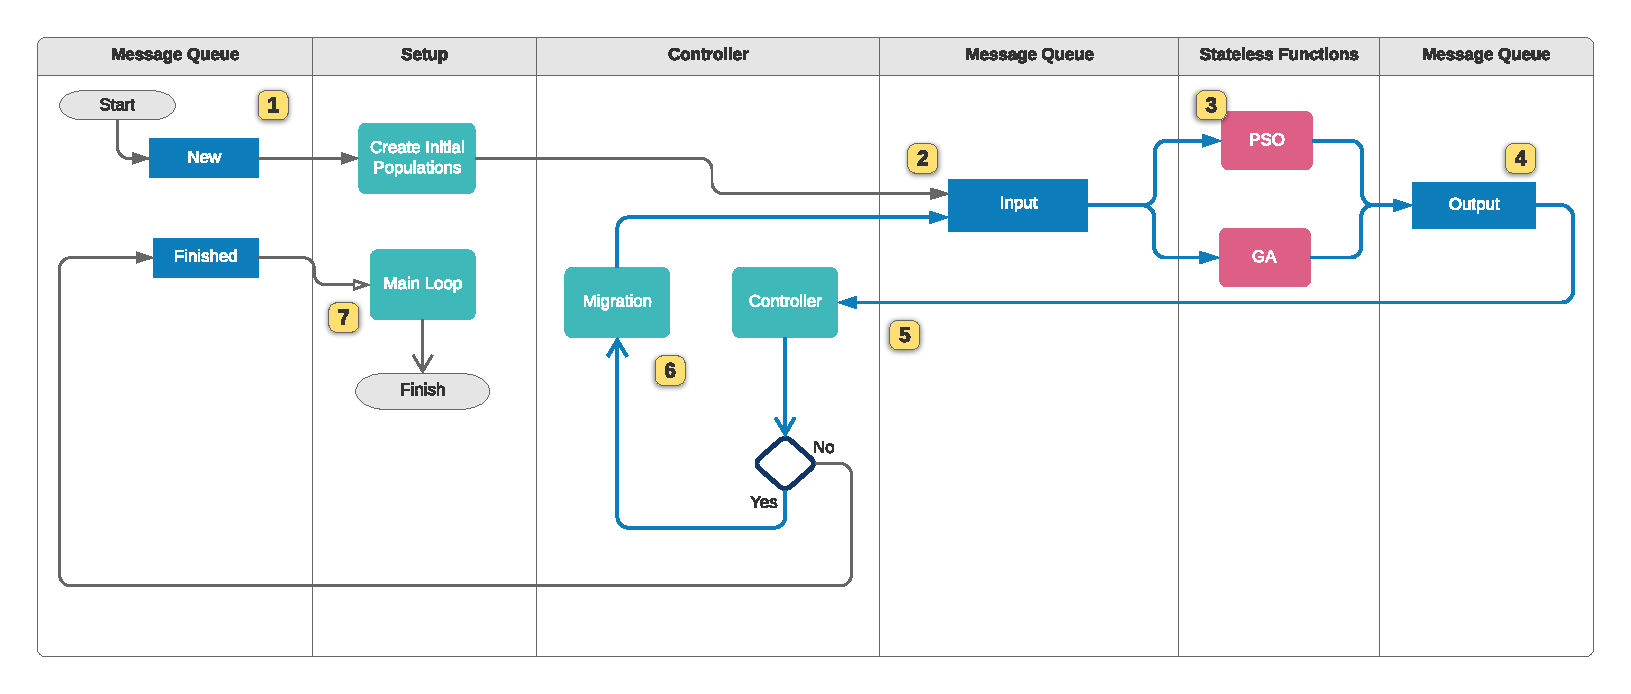
\includegraphics[width=\textwidth]{KafkEOsmall}
    \caption{The proposed general architecture, 
     showing each process in a swimlane, message-dataflow,
     message queues, and high-level tasks for each process.} 
    \label{fig:kafkEO}
\end{sidewaysfigure}

\subsection{Event Driven Model} 
\label{edm}
Based on a reactive architecture we proposed in a previous work
\cite{guervos2018introducing}, we now describe the general architecture shown in
Figure \ref{fig:kafkEO}. Again, we can explain the model using the analogy
of producers and consumers of messages. First, we can see that
there are two queues, one labeled \texttt{Input}, and the other one \texttt{Output}. In the diagram, 
push operations on a queue are represented by solid arrows connecting to the left side
of the queue box, and pull or pop operations as solid arrows leaving from the right side.
Also, the architecture has at least four processes indicated in the diagram as
swimlanes: First, the \texttt{Setup} process, responsible for the reading a configuration
file, and creating the initial populations. Second, the \texttt{Controller} process,
responsible for the migration between populations, and keeping track of the
iterations of the algorithm. The \texttt{Message Queue} process runs the \texttt{Input} and \texttt{Output}
queues. Finally, there is at least one \texttt{Stateless Function} process responsible
for running the isolated algorithms. In the example, two processes \texttt{PSO} and \texttt{GA},
are shown. 

The algorithm starts with the \texttt{Setup} process pulling a configuration message from
the \texttt{Experiments} queue, this is not shown in the diagram. The configuration message 
includes all the parameters needed to execute the algorithm, among other things,
the number of populations, the number of individuals, and the number of iterations
of the algorithm. We give more details about the configuration data structure
in Section \ref{experiment_flow}. % Missing  % added 
Once the configuration is read, we can follow the path of 
messages as follows:

\begin{enumerate}
\item In this step, the specified number of populations are created according to the 
parameters found in the configuration structure. The population at this moment is just
static data, including each individual inside. Each population includes a metadata
section where its algorithm and execution parameters are specified. For instance, 
for a GA, the mutation rate, type of crossover operator, and other values are indicated.

\item Each population is then pushed to the \texttt{Input} queue, so they can be consumed 
by Stateless functions responsible for the execution of the search.

\item One or more \texttt{Stateless functions} are constantly pulling population messages
from the \texttt{Input} queue. Taking the population data and metadata as parameters, these 
functions are responsible for the actual execution of the optimization algorithm. 
They take the current state of the population and run the algorithm for a certain 
number of iterations. 

\item Once they finish the execution, the population state
is packed again along with additional metadata about the execution of the algorithm.
The resulting populations are now pushed to the Output queue. Once finished, another 
population is pulled from the queue.

\item The \texttt{Controller} process is responsible for keeping track of the progress of 
the search. It pulls current populations from the \texttt{Output} queue, inspects the metadata 
and if an optimal solution has been found or the maximum number of iteration has been
reached it signals the stop of the execution. 

\item Otherwise, it passes the stream of messages 
to a migration process, where populations are mixed with each other. New populations 
are generated from this migration, and they are again pushed to the Input queue to continue 
in a loop. The \texttt{Controller} is also responsible of logging the metadata received with the
messages.  
\end{enumerate}

This reactive architecture has the following advantages:\begin{itemize}
\item 
An important aspect of proposal is the decoupling of the population and 
the population-based algorithm. It is common that in a classic island-based algorithm
each island is executed in a separate processing node, i.e. in a virtual machine, CPU,
or thread. In this case we can have just one processing node, or many nodes, each 
running a different search strategy, or using its own parameters. 
\item 
Also, the reactive controller gives designers more control over the multi-population algorithm.
In this process, designers can dynamically change the number of populations, population parameters,
and migration details on-the-fly.
\item 
Another advantage is that algorithm designers have many options for implementing this simple architecture. 
The same basic components can be implemented as a single multi-threaded program, or 
as a highly scalable serverless cloud application. Most modern languages include 
constructs for asynchronous programming using queues or channels, for a multi-threaded
execution.
\end{itemize}

\begin{figure}[ht]
    \centering
    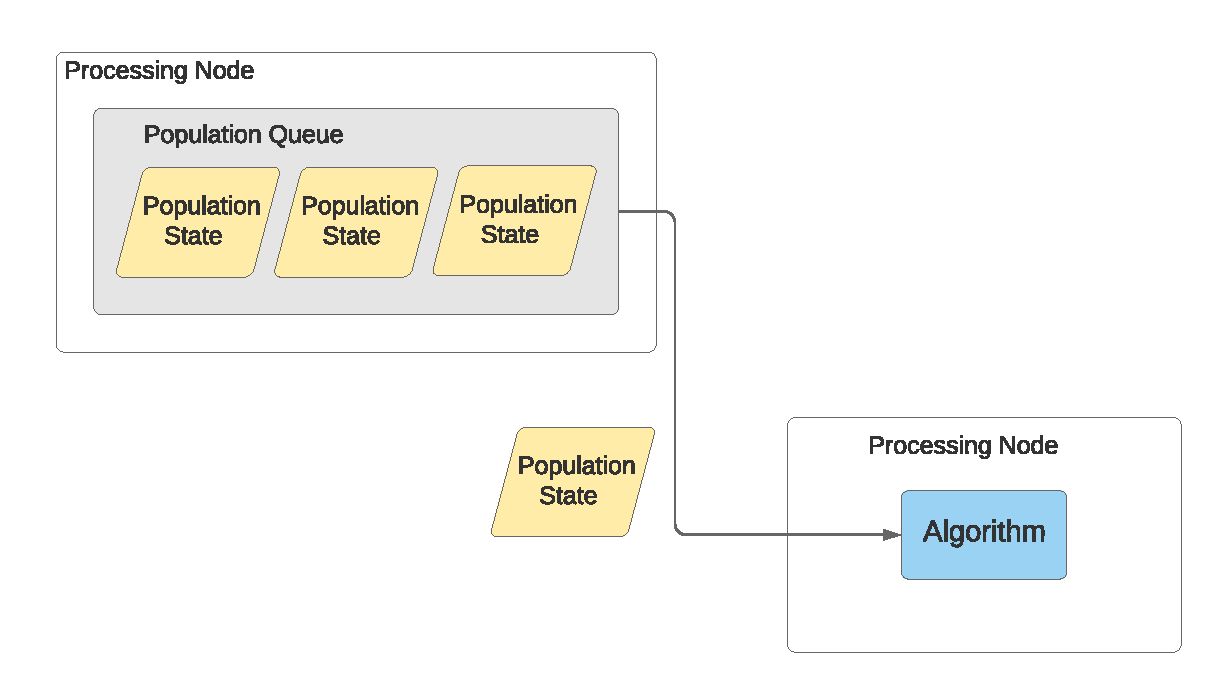
\includegraphics[width=\textwidth]{population_message}
    \caption{Population State and dataflow between processing nodes of a message-based algorithm.}
    \label{fig:population_message}
\end{figure}

On the other hand, there are several caveats as well:
It is more costly to move entire populations as messages than only passing certain individuals 
from a process to another. Designers must consider this cost when working with large
individuals, and if possible send populations using several messages, use compression or 
adjust the size of populations. Pool-based algorithms also suffer from this drawback, but 
web based implementations have been working with continuous optimization problems of 1000 dimensions.
But, in other cases this is not a viable approach. 

\begin{figure}[ht]
    \centering
    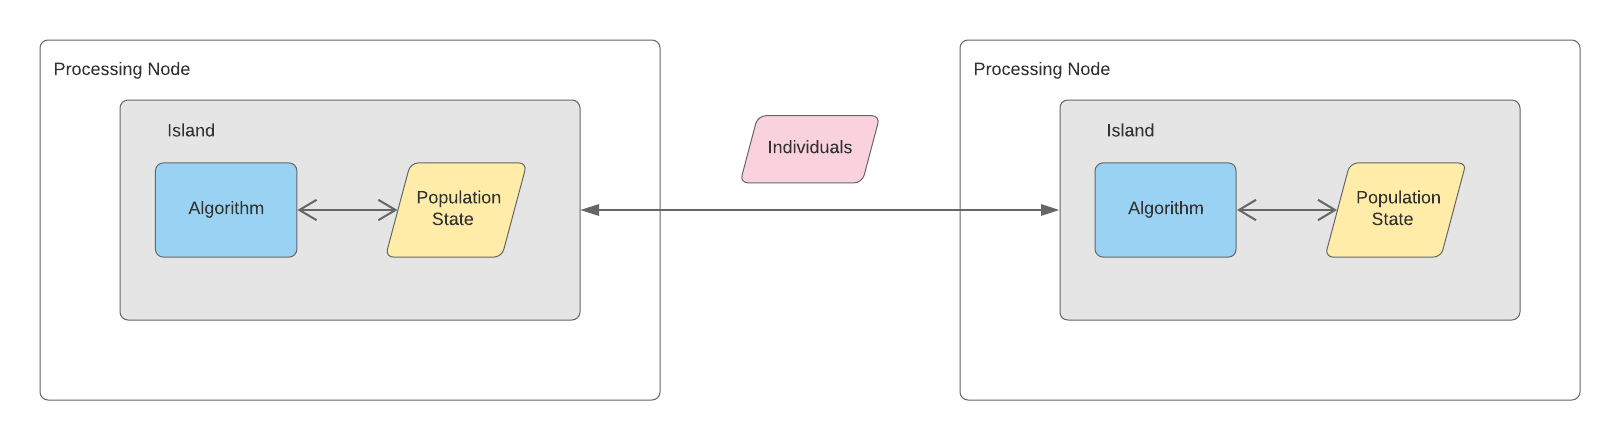
\includegraphics[width=\textwidth]{classicisland}
    \caption{ Population State and dataflow between processing nodes of a classic Island-based multi-population algorithm. }
    \label{fig:classicisland}
\end{figure}

\subsection{Comparison with Other Cloud-based Works} 
\label{comparison}

Next, we compare the message-driven architecture we presented against four other
proposals for multi-population algorithms found in the literature. We center the
comparison on the coupling and communication between the main components:
populations, processing nodes, and algorithms.  In Figure \ref{fig:population_message} we show the
main components of a message-driven architecture. We can see that the algorithm
and populations are separated, and the \texttt{Population queue} keeps the state
of populations. While algorithms only need the populations as parameters
for their execution.

% We need to add references to the respective papers - Mario

In contrast, in the classic island model shown in Figure
\ref{fig:classicisland}, algorithms are  population methods, and the same processing
node keeps both the algorithm process and the state of the population.  Other
processing nodes follow the same configuration and form of execution, and they
only pass specific individuals between them.  In this model, adding additional
processing nodes, on-runtime, can be more difficult, because they need to have
an addressing mechanism or simply be aware of these new nodes. This is
solved in part in Peer to Peer (P2P) evolutionary algorithms
\cite{juanlu:europar}, but coupling still exists, meaning that every
node must run the whole evolutionary algorithm and hold full copies of
its subpopulation. 

\begin{figure}[ht]
    \centering
    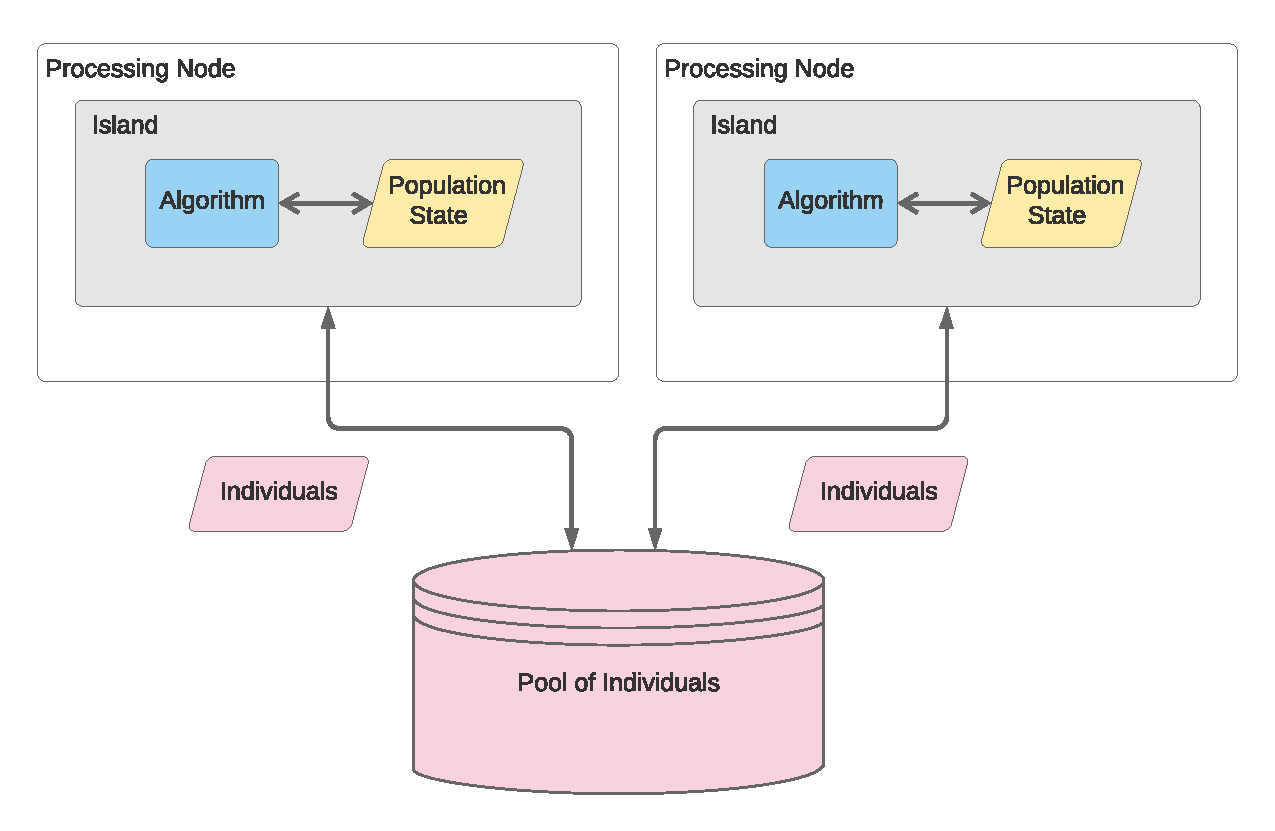
\includegraphics[width=\textwidth]{pool_island}
    \caption{Population state and flow of data between processing nodes of a Pool-based multi-population algorithm.}
    \label{fig:pool_island}
\end{figure}

A typical design pattern used to alleviate the above drawbacks is the use of a
central repository or pool of individuals that is available to all processing
nodes.  In Figure \ref{fig:pool_island} we show the main components of a pool-based
multi-population algorithm. Although algorithms and population state remains
coupled, now, processing nodes do not communicate directly with each other.
Instead, they interchange individuals with the pool. Communication between nodes
is not affected if the system adds or removes nodes because they do not know
about each other.  Since the state of the global population is stored in
external processing nodes, the system needs additional communication and
processing for keeping track of each population.

We show another pool-based approach in Figure  \ref{fig:population_pool}. In
this design, the global population is stored in a central repository, while
isolated algorithms take random samples of the global population and use this
temporal population as parameters. An advantage of this design is that the
sampling provides a type of migration between isolated populations. A problem
found is that when a processing node returns a population to the pool, the
state of the population is lost. But having the algorithm decoupled opens the
possibility of implementing the system using serverless functions.

\begin{figure}[ht]
    \centering
    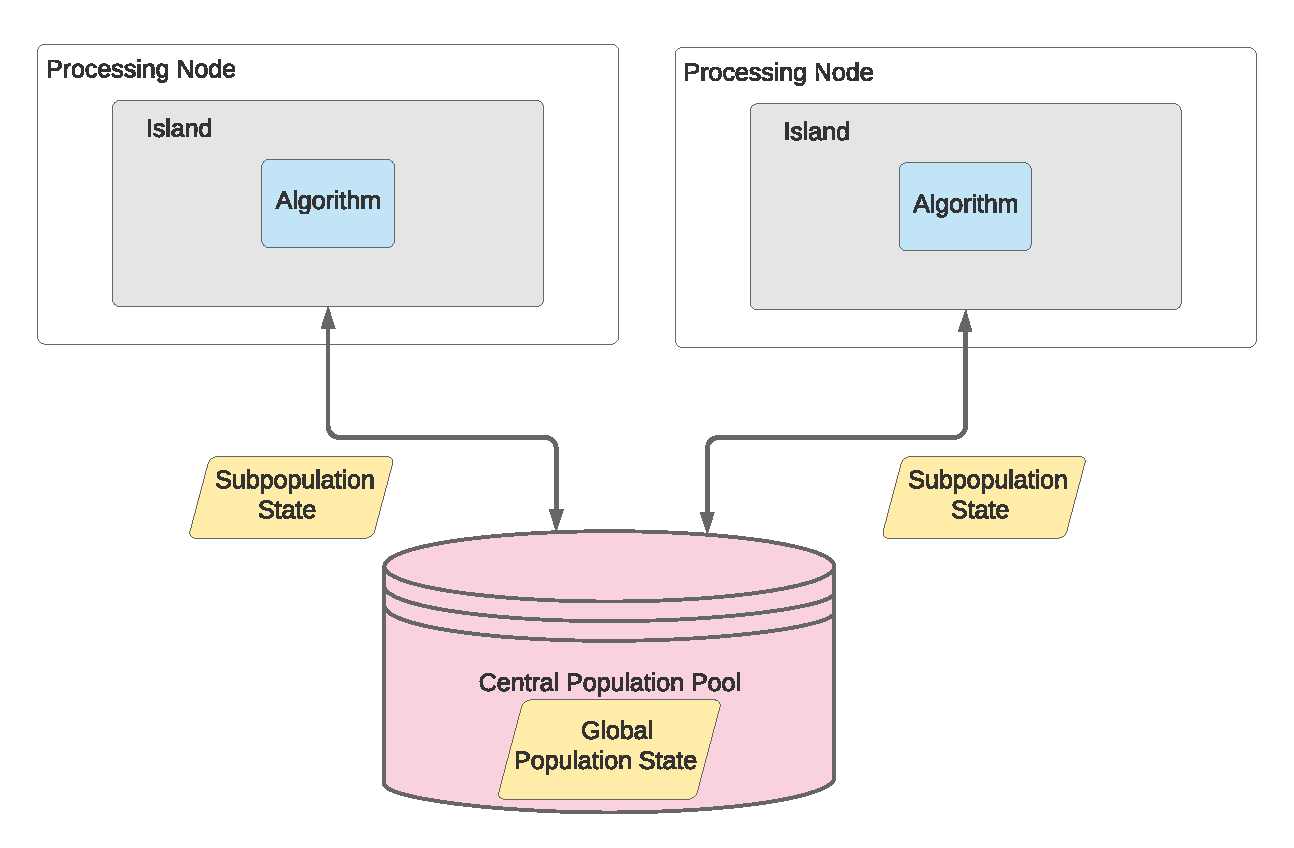
\includegraphics[width=\textwidth]{population_pool}
    \caption{Population State and dataflow between processing nodes of the EvoSpace algorithm.}
    \label{fig:population_pool}
\end{figure}


\section{Experimental Design of a Container-based Application} 
\label{docker}

We have mentioned several advantages of a cloud-native application for running
multi-population based algorithms, but there are in our experience, several
issues that make this approach more practical. % several issues that make it practical or useful instead? - JJ 
In general, cloud platforms have free-tiers    
for their services, and many offer academic discounts to students. But once we
pass to the pay-as-you-go tier, computing resources need to be
managed, and, where possible, its cost minimized.  First,
in many cases,  a credit-card is needed to guarantee the payment of the
resources consumed and someone responsible for assigning quotas and, more
importantly, special keys for using the cloud's API.  If these keys are
compromised or shared by their holders,  additional costs or administrative
procedures are in order. For those cases when a prototype platform is needed,
for instance, students developing a new algorithm variant or experimenting with
a published work, a container-based platform can be more practical. Container
technology enables researchers the local deployment of all the infrastructure
needed to run the experiments. Later, if needed, the same system could be
deployed to the cloud.

There are many advantages of container-based architectures over one
based on virtual machines. The main ones are architectural: it makes
the design of an application gravitate towards a set of decoupled
tasks, that use reactive, event based programming, to interact with
the rest of the application; containers hold micro-services that are
much easier to test, integrate and deploy. It also simplifies
the interaction APIs. Of course, that makes them more economical in a
pay-per-use cloud provider, but that is not the main reason why we
have chosen them in this paper; reproducibility of experiments and a
clear and idempotent description of the architecture through {\tt docker-compose} 
are the main reasons. 

In this section, we propose a design of a reactive container-based application
for executing multi-population based optimization experiments.  For the design,
we followed the design patterns highlighted in the previous section, and again
we can go back to Figure \ref{fig:kafkEO} and use it as a guide for explaining
the main components and their interactions. The containers used in this design will be explained next. 

\subsection{Message Queue Container} 
\label{message_container}

In this work, we implemented all message
queues in the Redis memory store. Early cloud architectures
\cite{de2017parallel} used queues for communication, although in that
case RabbitMQ was the chosen tool. Redis is faster, and also can act
as a data store from where we can control the state of the application.
Each queue is a Redis List object, and we use
the \texttt{LPOP} (left pop), and \texttt{RPOP} (right pop) commands for a queue like behavior.
In those cases where we needed a blocking behavior, i.e., when a process needs
to wait until a message is available, we used the blocking versions \texttt{BLPOP} and
\texttt{BRPOP}. Redis in-memory operation are very fast, and all of the above 
operations have a time complexity of $\mathcal{O}(1)$. We use the official 
\texttt{redis:alpine} container image from DockerHub.  

\subsection{Controller Container} 
\label{controller}

The controller is an essential component of the architecture (see Figure \ref{fig:kafkEO})
because it is responsible for maintaining the evolutionary loop. It takes newly
evolved populations from the \texttt{Output Queue}, mixes them,   and produces new
messages from the result. At the same time, it must keep track of two conditions
for ending the loop: the number of messages it has received reaches a maximum
value, or the error of the best solution goes below a specific threshold.  Finally, it
must filter out remnant messages from other experiments. Messages from other
experiments can remain in the queues because of the asynchronous nature of the
system.  We chose to implement the controller in Python but using an API
specialized in asynchronous event-driven programming over data streams.  
The open-source library is called Reactive Extensions (ReactiveX) for Python 
\url{https://github.com/ReactiveX/RxPY} an it is based on the Observer 
pattern \cite{gamma1995design} and functional programming.

\begin{figure}[ht]
    \centering
    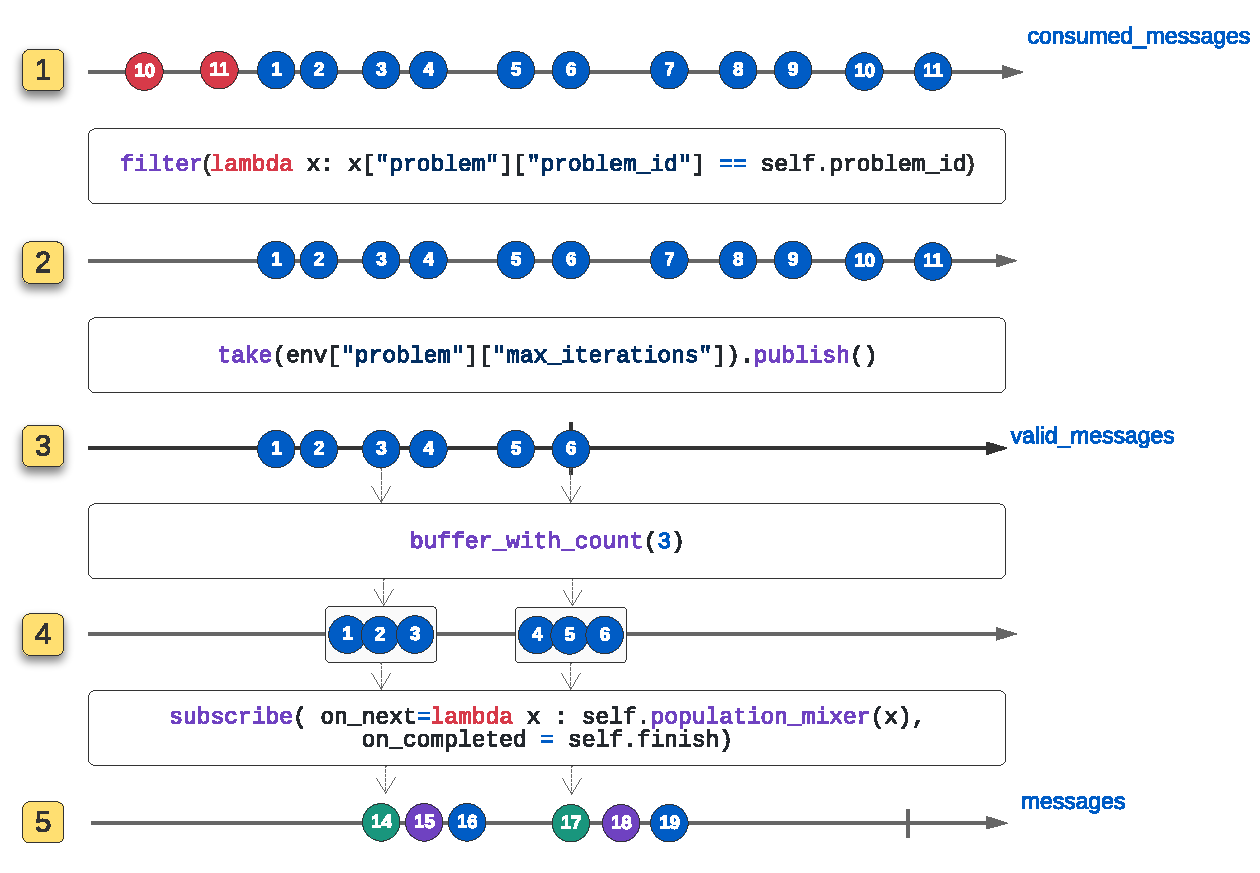
\includegraphics[width=\textwidth]{marble_controller}
    \caption{Marble diagram for the Reactive Python implementation of the Controller}
    \label{fig:marble_controller}
\end{figure}

In ReactiveX, an \texttt{observer} object subscribes to an \texttt{Observable} instance. 
Observables emit a sequence of items, and all the subscribed observers react to each emission. The
ReactiveX library includes several reactive operators that we can use to
transform and combine sequences of items. These operators provide reactive
extensions that allow us to compose asynchronous sequences together in a
declarative manner. In Figure \ref{fig:marble_controller}, we use a marble diagram to
represent the composition of \texttt{Observables} and reactive extensions operators. We
represent the timeline of an \texttt{Observable} as a horizontal arrow, which indicates
that time flows from left to right. In the diagram, items are represented as
marbles. The position of each marble indicates the point in time when they were
emitted by the \texttt{Observable}. Reactive operators are represented as text boxes,
showing the transformation to be applied. Normally, a transformation results in
another \texttt{Observable}, again emitting new results.  For asynchronous programming, 
this approach is more elegant than nested callbacks, that are more difficult 
to code and debug. 

Now we proceed to explain the reactive implementation of the controller.
In Figure \ref{fig:marble_controller}, we  have the following composition of Observables:

\begin{enumerate}
\item The controller continually pulls new messages from the \texttt{Output} 
message queue. These messages are instantly emitted by the  \texttt{consumed\_messages}
\texttt{Observable}. In this particular period, we can see that the stream receives 
two populations from another experiment, and are shown as two red marbles.  
The filter operator removes all messages that belong to a different experiment; 
in this case, we are only interested in blue marbles. 

\item The \texttt{max\_iterations} parameter indicates the number of populations that
are going to be accepted. When this number of messages is reached, we must
end the loop. In this example, \texttt{max\_iterations = 6},  the take operator 
assures that only 6 messages are received. After the \texttt{Observable} emits 
the sixth message, it triggers the completed event.

\item Many observers can be subscribed to the \texttt{valid\_messages} \texttt{Observable} because it
emits all the valid items. At the moment, there are to additional methods
subscribed that we are not showing, one for logging and the other for monitoring
the search.

\item The   \texttt{buffer\_with\_count(3)} operator, waits until it receives 
three valid messages to emit a single message that contains a list with
the previous three. The \texttt{population\_mixer}  method requires that list to mix them. 
In our previous work, we needed a local buffer for storing a certain 
number of populations to mix them with others. This design has the advantage
of not needing extra memory, and it integrates better with the reactive paradigm.
A possible disadvantage can be that it only mixes contiguous populations,
but this can be mitigated with a larger buffer.

\item The \texttt{population\_mixer} receives a list of three populations,
let us say [A, B, C], and calls the migration method shown in
Algorithm \ref{alg:migration}  for [A, B], [B, C] and [A, C]. 
The migration algorithm sorts both populations and generates
a new population containing the best half from each.
This migration method is similar to those used successfully in previous 
works on pool-based algorithms \ref{fig:pool_island}.  
Finally, the method pushes the new populations to the 
\texttt{messages Observable}. From there, a
\texttt{publish(population)} observer is responsible for pushing
the newly generated populations back to the \texttt{Input} message queue.
\end{enumerate}

\begin{algorithm}
    \caption{Migration}
    \label{alg:migration}
    \begin{algorithmic}[1]
        \Procedure{cxBestFromEach}{$pop_1,pop_2$}
            \State $pop_1.sort()$
            \State $pop_2.sort()$
            \State $size\gets min(len(pop_1), len(pop_2))$
            \State $cxpoint\gets (size-1)/2$
            \State $pop_1[cxpoint:]\gets pop_2[:cxpoint+2]$
            \State \textbf{return} $pop_1$
        \EndProcedure 
    \end{algorithmic}
\end{algorithm}



In the next section, we follow the algorithm flow and describe the 
implementation details of the \texttt{worker} containers. 

\begin{figure}[ht]
    \centering
    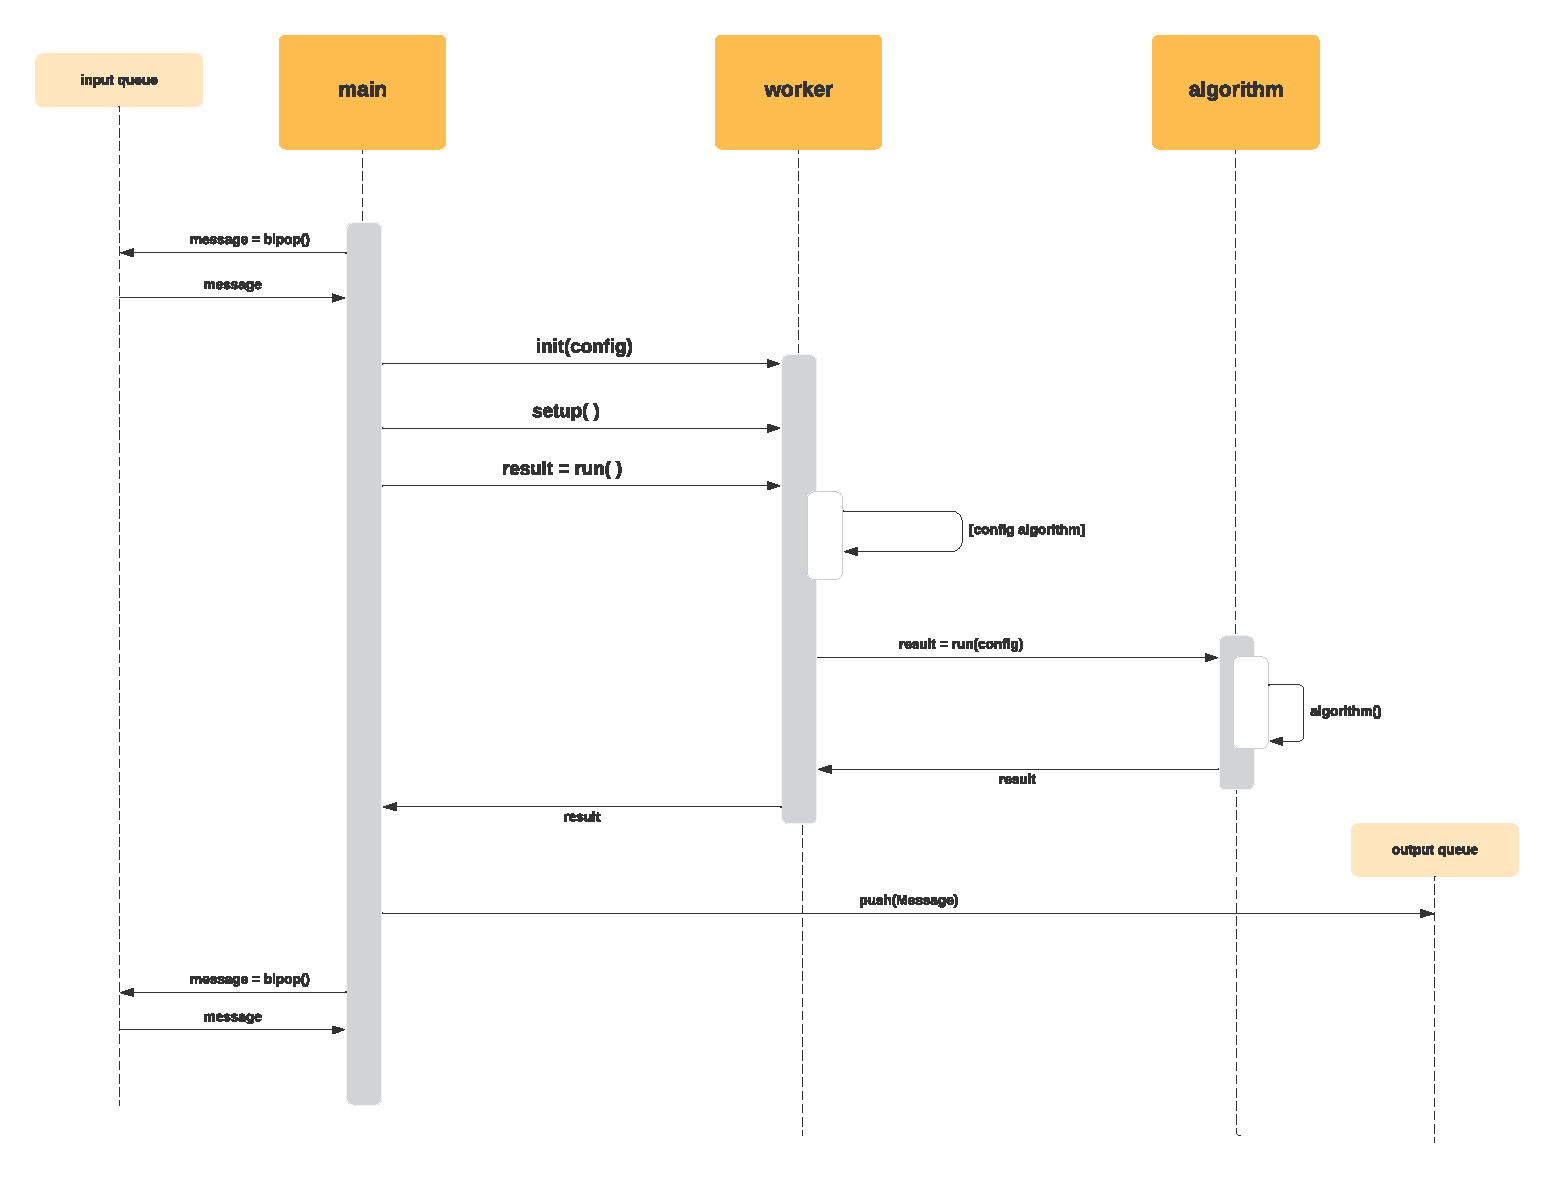
\includegraphics[width=\textwidth]{worker_new}
    \caption{Serverless function implementation details. Showing the worker algorithm in each container}
    \label{fig:worker}
\end{figure}



\subsection{Worker Containers} 
\label{workers}

Worker containers include a Python script called \texttt{main.py} running an
infinite loop, continually trying to pull a new population to work on it. Once
\texttt{main.py} receives a message containing configuration data, it creates a
worker object responsible for initializing and running the specified stateless
function (i.e., GA or PSO) with the population and configuration in the message.
Once the function returns the evolved population, the
the main script pushes the results to the \texttt{Output} queue, and continues
the execution to the infinite loop. This process is shown in Figure
\ref{fig:worker}.

\section{Workflow for Reproducible Experiment Design in EvoSwarm} 
\label{experiment_flow}
% Changed the section title to give more focus on reproducibility - M
% You can't start with this. Explain what this section is about, and link it with 
% the previous one. Maybe it's better to create a big section with "Experimental setup", 
% and make this a subsection, with subsections becoming subsubsections - JJ 
% done - M 

An essential goal of our EvoSwarm application is to allow researchers the
description and orchestration of reproducible multi-population experiments.
Following the application design described in the previous section, we now
present the workflow of an experiment's entire life-cycle viewed from the
perspective of the two roles users can play. On one side is the user role that
designs and runs experiments and, on the other, the role of a developer of
algorithms. The scenario presented in Figure~\ref{fig:experiment_flow} shows the
workflow of an experiment in Evo\-Swarm the two roles users can play. The first
step is to develop the search strategy algorithms that are going to be used by
the multi-population algorithm; algorithm developers do this. Then users are
responsible for the configuration and deployment of the resources needed for the
experiment. Once the application is running, users can start one or several
experiments, monitor the execution, and analyze the results. Depending on the
type of experiment executed, users could have additional needs, in this case
there are additional scripts for processing the results of experiments to be
used with the COCO framework. In the next sections, we give more details about
these roles and their workflows, and at the end we present a proof-of-concept example of a
reproducible experiment in EvoSwarm.

%\begin{itemize}
  % Question move to here for the moment, I mention this in this intro. - Mario

%  \item Can EvoSwarm as a cloud-native, container-based application,  be deployed
%  locally or in the cloud by just specifying the configuration of container images
%  and resources to an orchestration service? 
%\end{itemize}

  

\begin{sidewaysfigure}
    \centering
    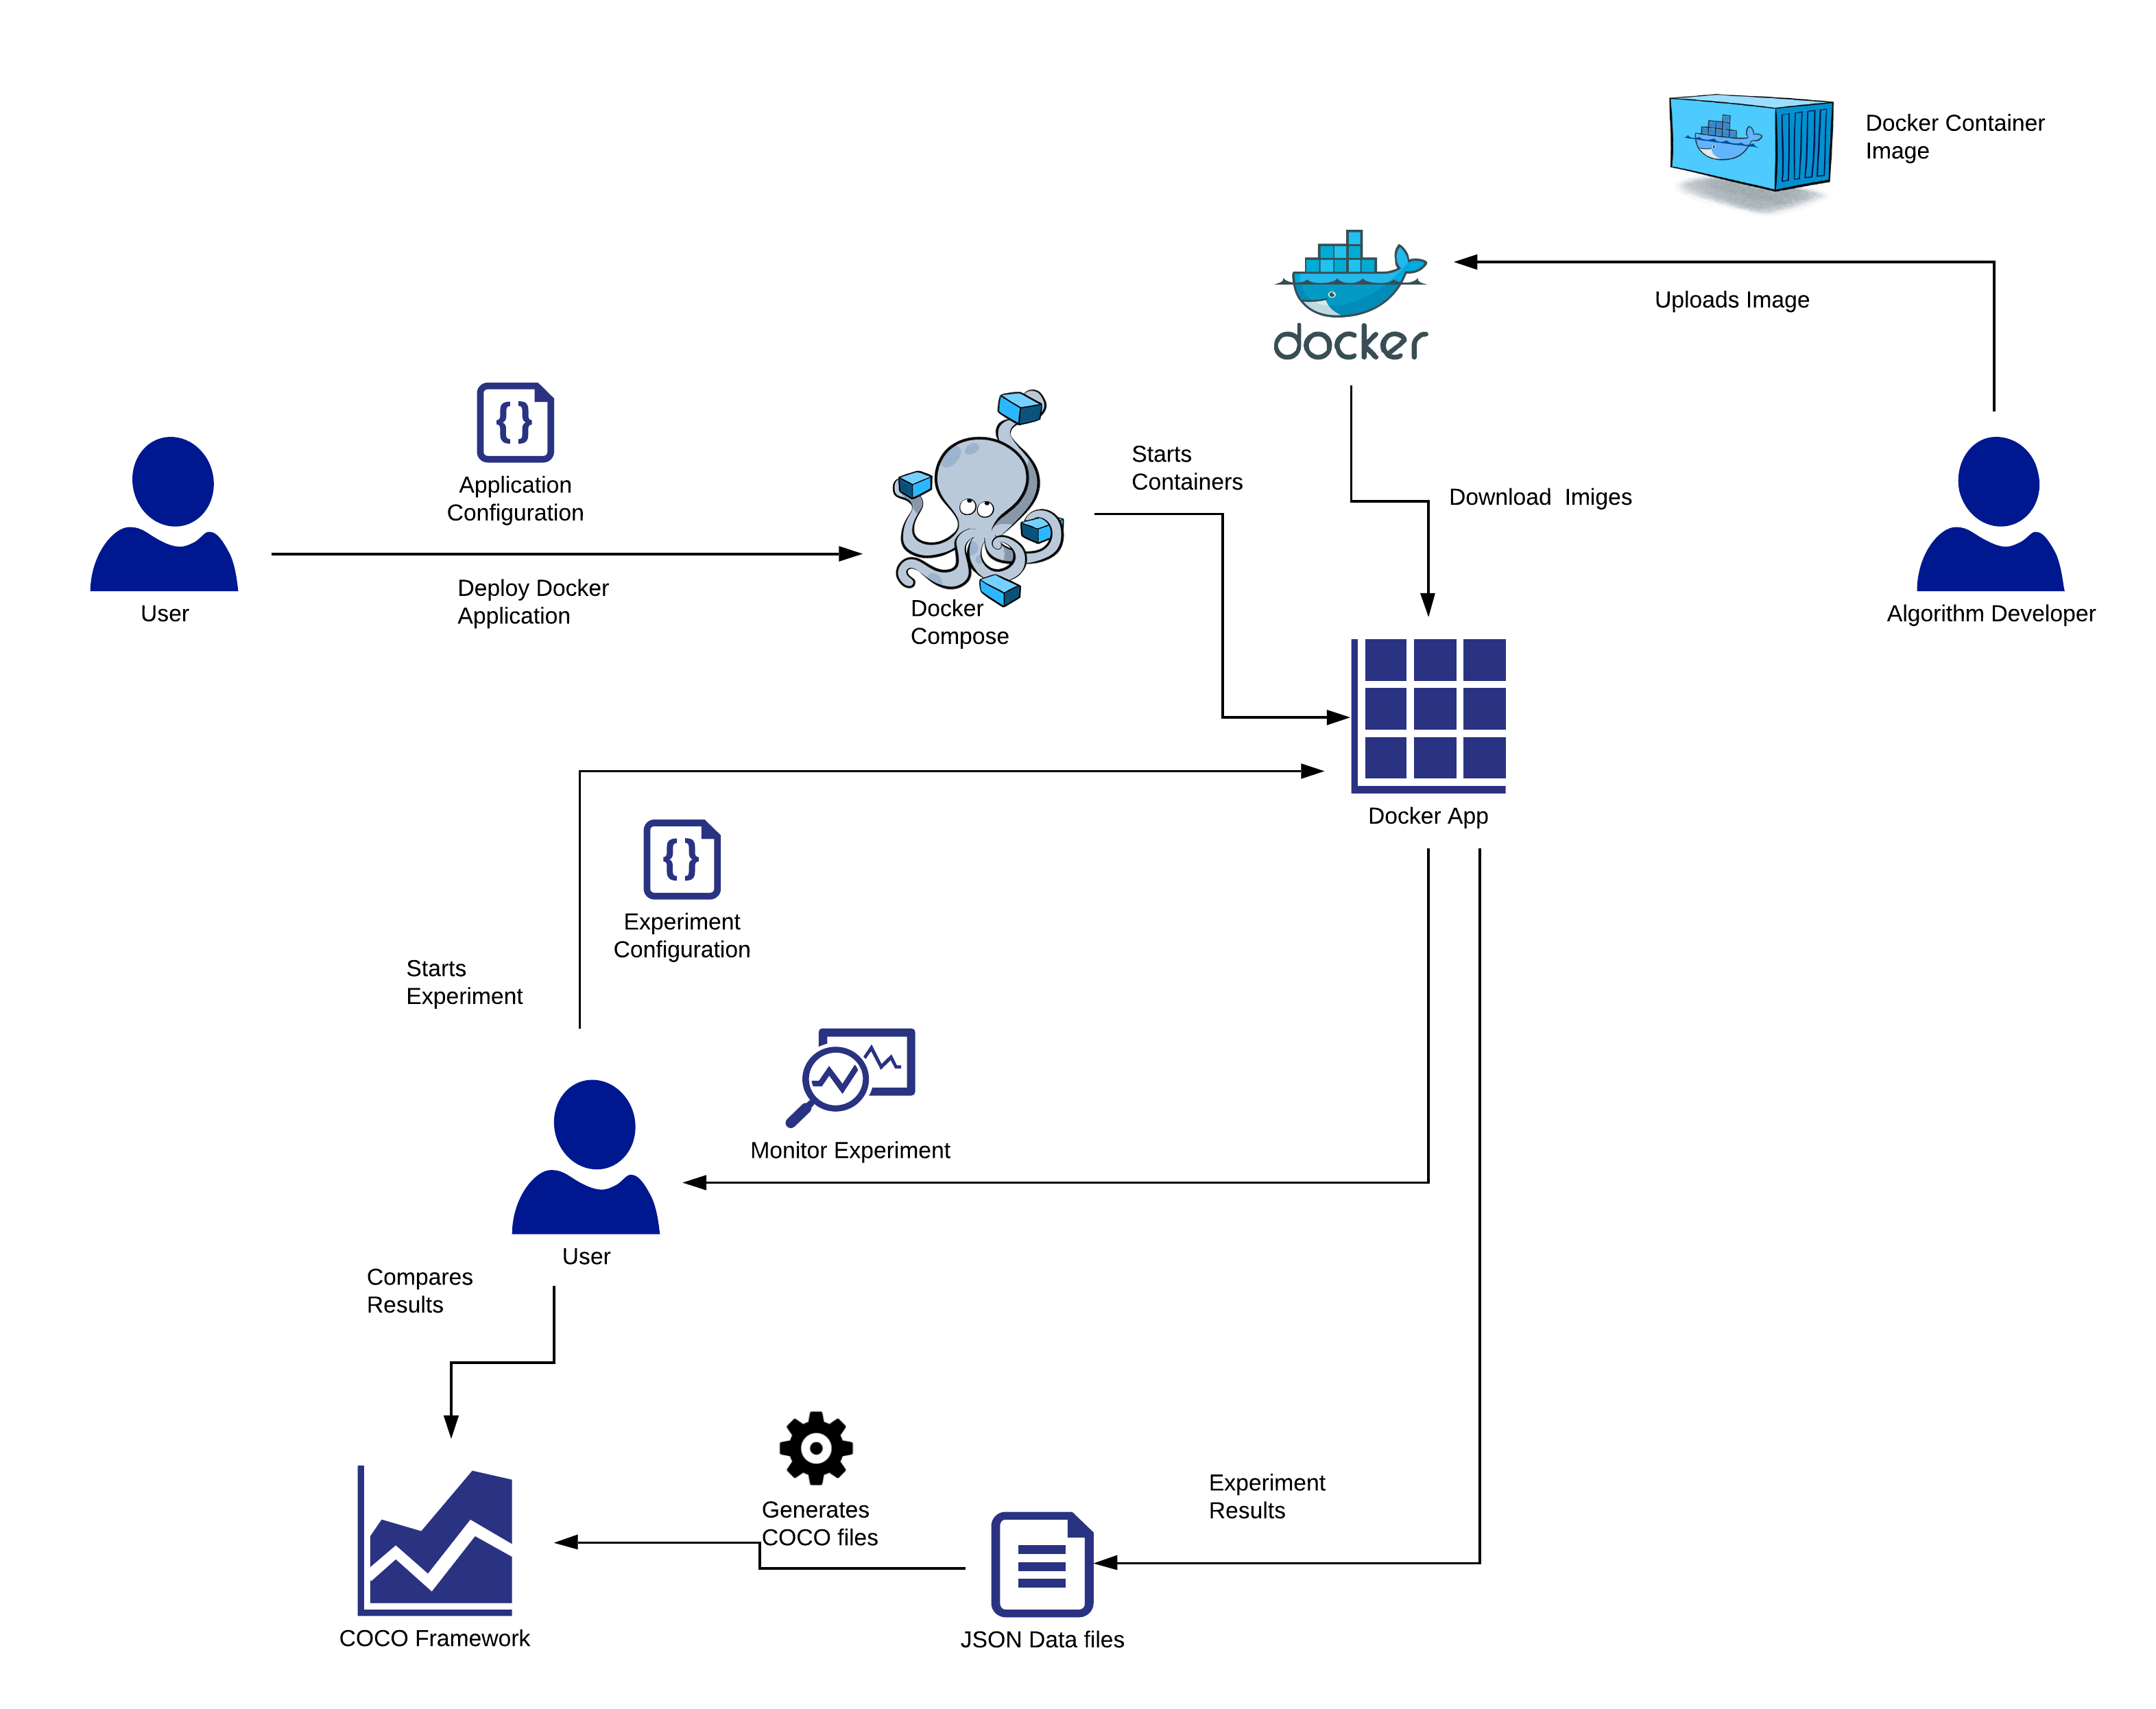
\includegraphics[width=\textwidth]{experiment_flow}
    \caption{EvoSwarm Workflow}
    \label{fig:experiment_flow}
\end{sidewaysfigure}

\subsection{EvoSwarm from the Developer Point of View} 

Developers can add new algorithm as stateless functions in
several ways and with two levels of integration. In the first level of
integration, the algorithm execution is not dependent on an initial
configuration created in the setup, and it only needs to take messages from the
input queue and return the modified population to the output queue. On the
second level, the algorithm receives a configuration from the initial setup,
specifying the initial algorithm parameters. We show an example of the configuration
file received by workers in Listing \ref{code:config}  in which we abbreviated
the population key (the ellipsis is used instead). The message includes the current state
of the population, together with data about the problem, algorithm,
and its parameters. 

\begin{lstlisting}[language=Python, caption = Configuration message example, label=code:config]
{"problem":{
  "name":"BBOB","instance": 1,"error":1e-8,"function":4,
  "dim":3,"search_space":[-5,5],
  "problem_id":"1515-4-1-3",
  "max_iterations": 20,
  "population":[
          [ -3.323452321611405, 
             2.593007989886873, 
             3.001112341167673],
             ...
          [ -2.22e343232411405, 
             2.593007989886873, 
             2.0011025031167673] 
          ],
  "population_size": 100,
  "algorithm": "GA",  
  "params":{
      "GA":{"crossover": { "type": "cxTwoPoint", 
            "CXPB_RND": [0.2, 0.6], "CXPB": 0.26},
             "mutation": { "MUTPB_RND": [0.1, 0.3], 
             "indpb": 0.05, "sigma": 0.5, 
             "type":"mutGaussian","mu":0,"MUTPB":0.12},
             "selection": { 
               "type": "tools.selTournament", 
               "tournsize": 2 },
               "iterations": 50},
       "PSO": {"Vmax":5,"wMax":0.9,"wMin":0.2,
               "c1":2,"c2":2,"iterations":50 } 
    },
  "experiment":{"type":"benchmark","experiment_id": 1515}
  }
}
\end{lstlisting}

In the case of the first level of integration, developers
can implement a new stateless Docker container following
the description in the previous section (\ref{workers}). The worker
container executes a daemon that continuously pulls messages from the input queue
on the Redis host specified as an environment variable {\texttt REDIS\_HOST}. If the new
population-based algorithm is written in Python, developers can base the new
implementation on the provided worker container image, adding a new algorithm
function and worker and modifying the \texttt{main.py} file. 
The worker must include a constructor with the configuration dictionary 
(see Listing \ref{code:config}) as the only parameter, and call a the new function 
with the required parameters, unpacking them from the configuration dictionary if necessary.
All the code of the EvoSwarm Application is published with the open source MIT license.

If developers use an existing library for population-based algorithms, they need
to change the standard model of execution, that creates first a random
population because, in this case, the algorithm needs to start with the
population provided as a parameter. Depending on the evolutionary (or other) algorithm library used,
it may be required to extract the population from the
JSON message and replace the population object created by the default library implementation. For
example, the DEAP library we used for the GA algorithm, creates the type of the
population at runtime (i.e., bit, float), so we have to replace the population
once DEAP created it. In the case of EvoloPy, the PSO method directly uses a
list of floats for storing the swarm, so we just added a parameter to receive
the population as a list of floats. Both libraries store information about each
iteration, so we just read it and put it in the format required.
Again, the state of the population must be encoded as a JSON message to be
returned as a result, with additional data as
depicted in Listing \ref{code:result}. The output message contains the id of the
worker container together with records giving information about each iteration
of the algorithm, including the best solution found. The controller uses this
information to track the execution of the algorithm and keep a log in the Redis
container for posterior analyses.

\begin{lstlisting}[language=Python, caption=Fragment of an output message, label=code:result ]
{
"time_stamp": 1588455316.698875,
"evals": [
  {
    "gen_num": 0, "best_fitness": -259.96925945939404,
    "best_solution": [ -4.9446848321611405, 
                        2.593007989886873, 
                        2.0011025031167673],
    "num_of_evals": 17
  },
  {
    "gen_num": 49, "best_fitness": -419.47555780783347,
    "best_solution": [ -0.9165294450108963, 
                        2.291966676472422, 
                        1.8527006568795485],
    "num_of_evals": 28
  }
],
"worker_id": "4f5eb12e-8278-40de-b0f3-4ac18171566d",
"message_counter": 1,
"message_id": "cbcd2e82-e232-4818-8aec-2cd072c7cfe9",
"best_score": -419.47555780783347
}
\end{lstlisting}

For the secondary level of integration, developers need to add code to the setup
container to specify additional configuration options. For instance,
in the current configuration message (see Listing \ref{code:config})
workers executing a GA, initialize the mutation and crossover 
probabilities randomly from a specific range of values. Users specify
this range on the experiment configuration. 
Migration between populations is independent of the type of algorithm, as the
controller treats messages as the same type of objects. But developers could
also change the controller to specify new rules of operation, for instance, to
change the type of migration depending on the algorithm. 
For example, in the case of swarm-based algorithms,  migration between  
populations (swarms) can follow a topology, indicating valid connections 
between them (i.e., ring or hypercube). The controller
can apply these rules selectively only to swarm-based algorithms. 
In general, these configuration options will be algorithm and library specific. 

On either level of integration and after making the changes outlined before,
algorithm developers can upload the container 
definition or images directly to a public repository like DockerHub. 

Another option is to upload the container image definition (Dockerfile) to GitHub and
define a trigger to re-upload the image to the registry after an update. Having
images publicly available can contribute to the reproducibility of experiments.
Moreover, having more algorithms available can benefit researchers trying to
compare against other algorithms or increase the diversity of their algorithms
by adding more search methods. Finally, in some cloud services, having hosted
images is a requirement, as it is the case of Amazon ECS.

Moreover, public repositories have the functionality for documenting, sharing,
and tracking different versions of both images and image definitions by using
tags. This infrastructure supports the objective of the paper, which is to
contribute to the reproducibility of experiments and platform independence.

\subsection{EvoSwarm from the User Point of View} 
\label{sec:evoswarm:config}

The user role is responsible for
editing the {\tt docker-compose} configuration files that reference the images created
by developers. To deploy the application, he or she needs to edit the {\tt
docker-compose.yml} file to specify the type and number of containers required
for the experiments. Then, the {\tt docker-compose} application is responsible for
starting all the containers, and downloading new versions if it is necessary,
by executing the command {\tt docker-compose up}  inside the EvoSwarm directory.


After starting the application, users can push several Experiment Definition 
files at a time and start monitoring the current execution in the terminal.
After an experiment is finished, the user must execute another script
that takes as argument the experiment id to generate a collection of files containing all the
data generated by the experiment, again in a JSON format. An example of an 
experiment definition is shown in Listing \ref{code:exp}. We give more details about the 
data contained in the file in the next section. Users can use these files 
to analyze and plot experiment data.  Python
scripts are included in the repository to plot the running times for the
experiments, and all other plots used in this paper;  there is also a script to
generate the files needed by the COCO framework \cite{hansen2016coco}, which can generate standard
comparisons against other methods.


\begin{lstlisting}[language=Python, caption=Experiment definition example, label=code:exp]
{
"DIM_CONFIGURATION" : 
 {
 "10":{"GEN":50,"POP_SIZE": 70,"MAX_ITER":30,"MESSAGES":10},
 "20":{"GEN":66,"POP_SIZE":100,"MAX_ITER":30,"MESSAGES":10},
 },
"GA_WORKER_RATIO" : 0.5,
"FUNCTIONS": [4],
"DIMENSIONS" : [10, 20],
"CXPB_RND": [0.2, 0.6],
"MUTPB_RND": [0.1, 0.3]
}
\end{lstlisting}


\subsection{Deploying to a Cloud Provider}
\label{cloud-aws}


EvoSwarm describes the deployment of loosely coupled processes in a consistent
and portable way. The term cloud-native describes these container-based
environments because we can deploy them on an infrastructure that abstracts the
underlying compute, storage, and networking primitives. This infrastructure does
not need to be a cloud provider; it could be a developer's laptop, a single
server, or a production environment. In this section, we give specific details
about how we deployed EvoSwarm in a cloud-setting for running the experiments
within this paper. Running the cloud-native application in the cloud has the obvious
benefit of a multi-instance deployment, where we can run containers in several
instances executing at the same time, not only in a single machine.

When we deploy a cloud-native application to a cloud provider, there
are, among others, two options to choose from:

\begin{description}
  
  \item[A Kubernetes cluster] provides auto-scaling and management of
  containerized applications, but it needs additional configuration for
  provisioning and its cost might be higher. All major cloud-providers have Kubernetes services. This option
  was used by S. Zhao et al. \cite{zhao2019cloud} to run a multi-island
  algorithm, and Dziurzanski et al. \cite{dziurzanski2020scalable} later refined
  it.


  \item[A container orchestration service] these services are compatible with {\tt docker-compose}
    files for configuration and provide transparent provisioning. Examples of these
    services are Amazon Elastic Container Service,  Red Hat Openshift
    (which is also open source), and Marantis Docker Enterprise.
    Salza et al. \cite{salza2019speed} tested this option by using CoreOs cluster. 

\end{description}

%\subsubsection{Setup} % Even if it's a sub-sub section, flesh this out ... - JJ
%\label{setup:local-cloud}

We chose the second option, that is, a container orchestration service, and
deployed the EvoSwarm application in Amazon Elastic Container Service (ECS),
since it needs fewer changes in configuration (from deploying it locally using
{\tt docker-compose}) and it is has a lower cost than the Kubernetes
alternative.

We can define an ECS cluster directly on the AWS Elastic Cloud VMs or through the
AWS Fargate service. Fargate is a serverless compute engine for containers that
provides automatic provision and management of AWS ECS resources. With this
service, calculating the cost of execution is simplified because users only
specify the computing units and memory for the application, instead of every
component. However, AWS Fargate is not suited for an experimental setting because
many of the details are out of user control. For this reason, we chose the
alternative of using a cluster of EC2 containers. The drawback is that we need to manually
provision the  EC2 containers, networking, and group permissions for each
experimental setup; for instance, when going from 2 to 8 workers, we need to increase the
number of EC2 instances to meet the required amount of CPU units.

Multicontainer applications are deployed to ECS as tasks, and a single cluster can run multiple tasks in
parallel. Using the ECS CLI, we can provision a cluster with a configuration file
specifying the computing resources needed. We can also specify the configuration of a task 
by using a task definition file (see Listing~\ref{code:ecs}) in YAML format.
The main attributes are the {\texttt cpu\_shares} indicating the CPU units
assigned, in this case $2048$, and the network configuration; in this case we have two private 
subnets and a security group in this configuration. When deploying to EC2 containers, these requirements
need to be supported by the currently available cluster. For instance, we need to have all 
the CPU units required by all tasks, if they are not available, the task initiation will fail.

The complete task configuration is generated by the {\texttt ecs compose command} that uses a {\texttt docker-compose.yml} file to generate 
the configuration on-the-fly. For example to deploy the controller, setup and Redis 
containers we used the file in Listing ~\ref{code:compose}.

Each container is defined as a {\texttt service} ({\em task} in AWS terms), with the following attributes: {\texttt image},
that reference the container images we have published in Docker hub
\url{https://hub.docker.com/u/mariosky}, open {\texttt ports}, a {\texttt command} to be executed at
startup, configuration for the AWS {\texttt logging} service, and finally {\texttt environment}
variables used by code running inside containers.

\begin{figure}[h!tbp]
  \centering
  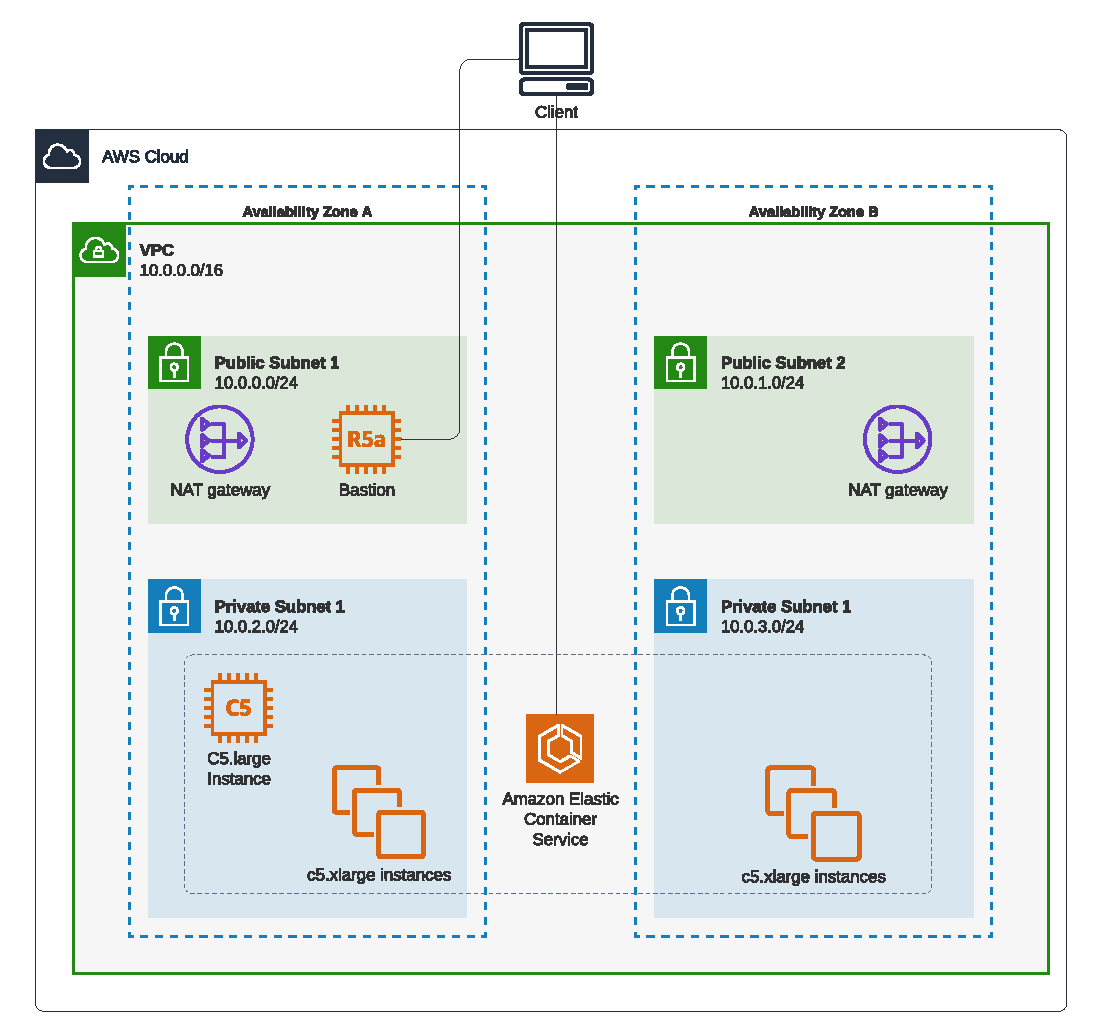
\includegraphics[width=\textwidth]{aws_ec2}
  \caption{AWS EC2 configuration for the deployment of EvoSwarm containers.
  }
  \label{fig:aws-configuration}
\end{figure}

Figure \ref{fig:aws-configuration} shows the basic EC2 configuration used for the deployment
of experiments. We selected three types of EC2 instances according to our needs; the  
{\texttt setup}, {\texttt controller}, and {\texttt redis} containers do not demand many resources
and we do not need to scale them as the amount of parallel workers are increased. They run in a
single {\texttt C5  High-CPU large} instance. With the available 2048 CPU shares divided as follows:
{\texttt setup} (128),  {\texttt controller} (896),{\texttt redis} (1024). With this assignment 
the {\texttt redis} container gets a dedicated vCPU, needed because it is the most demanding 
task of the three. We assigned 2048 units to each {\texttt worker} container, and using a more 
capable {\texttt C5 High-CPU XLarge} instance,  with 
four vCPUs and 4096 CPU shares, with this configuration each worker gets a pair of vCPUs.  
We scaled the number if instances as needed, using one instance for every two {\texttt worker} containers. 

Because all these instances run in a private subnet, we also
run a Bastion instance, that is, a specially protected network node, in a public subnet, from where we send the
commands to execute the experiments
and later collected the results. We connected to this instance through a {\texttt ssh} session from 
our personal workstation. This is a {\texttt R5AD Large} instance, selected with 75GiB of storage, needed for
keeping the logs, and more memory (16GiB) for processing the logs in memory. The details these EC2 instances 
and their cost at the time of writing are shown in Table \ref{tab:ec2}.


\begin{table}[h!tbp]
  \small
  \caption{Details of EC2 instance types used in our deployment}
  \label{tab:ec2} 
  \centering
  \small
  \begin{tabular}{|l|l|r|l|l|}
    \hline
    Name & Memory & vCPUs & Storage  & Cost \\ \hline
    R5AD Large	&	16.0 GiB	& 2 vCPUs	& 75 GiB 	& \$0.131000 hourly \\ \hline
    C5 High-CPU Large	&	4.0 GiB	& 2 vCPUs	& EBS Only 	& \$0.102000 hourly \\ \hline
    C5 High-CPU XLarge	&	8.0 GiB	& 4 vCPUs	& EBS Only 	& \$0.154000 hourly \\ \hline
  \end{tabular}
\end{table}

\begin{lstlisting}[caption=ecs-params.yml , label=code:ecs]
  version: 1
  task_definition:
    ecs_network_mode: awsvpc
    services:
      worker:
        cpu_shares: 2048
  
  run_params:
    network_configuration:
      awsvpc_configuration:
        subnets:
          - "subnet-0ca2a542bbd74239e"
          - "subnet-0dfd367b5ca531b07"
        security_groups:
          - "sg-0681c18469874b391"  
\end{lstlisting}

\begin{lstlisting}[caption={docker-compose.yml for setup, controller and redis containers}, label=code:compose]
  version: '3'
  services:
    redis:
      image: "redis:alpine"
      ports:
        - "6379:6379"
      logging:
        driver: awslogs
        options:
          awslogs-region: us-west-2
          awslogs-group: docker-logs
          awslogs-stream-prefix: redis
  
    setup:
      image: mariosky/setup
      command: python experiment.py
      environment:
        PYTHONUNBUFFERED: 1
        REDIS_HOST: localhost
      logging:
        driver: awslogs
        options:
          awslogs-region: us-west-2
          awslogs-group: docker-logs
          awslogs-stream-prefix: setup
        
    controller:
      image: mariosky/controller
      command: python controller.py
      environment:
          PYTHONUNBUFFERED: 1
          REDIS_HOST: localhost
      logging:
        driver: awslogs
        options:
          awslogs-region: us-west-2
          awslogs-group: docker-logs
          awslogs-stream-prefix: controller
  \end{lstlisting}




%


The complete configuration files are available at public GitHub repository 
\footnote{\url{https://github.com/mariosky/EvoSwarm/tree/master/aws-EC2}}, and
they are used on the next section to carry an extensive evaluation of the framework.
Again, each configuration describes the deployment of containers in a consistent
and portable way, an it was used in each phase of the life cycle, from
development through testing to production independently on the kind of
infrastructure.


\section{Experimental Study} 
\label{setup} % To be renamed 


In the previous section, we have described an option for an EvoSwarm deployment that can be used by 
the public to create reproductive research in the cloud; in this section we are
using the same framework to learn if the proposed solution can efficiently
improve the scalability and performance of population-based optimization
algorithms. 
Hence, in the following sections, we provide answers to the following questions:

\begin{itemize}
\item Can we improve the execution time of the algorithm by adding populations
 and serverless functions (workers)  to the system and, in particular,
 what is its effect on the scalability of the system? % Improve with respect to what? Single population? 
                         %Please explain carefully the issues and how scaling is related to the number of populations. - JJ
                         % The question could be that, How scaling is related to number of populations and workers in the system ? - M
 
\item Does having a multi-population enabled platform, with heterogeneous populations and
the support for mixing search strategies,  increase the performance of the
search by needing fewer function evaluations than a homogeneous setting? 
% Moved reproducibility question from here - M

\end{itemize}

Section~\ref{sec:exp1} is devoted to answering the first question, and Section~\ref{sec:exp2} to the second.
Next, we describe the general experimental setup designed to answer
both questions.

\subsection{General Experimental Setup} 
\label{sec:general-setup} 

To validate these questions, we used benchmark functions from the Continuous
Noiseless BBOB testbed, which is part of the Comparing Continuous Optimizers
(COCO) framework \cite{hansen2016coco}. The testbed includes 24 real-parameter,
single-objective benchmark functions, and the capability to provide additional
instances of each function. Each instance of a function has a different optimal
value. The standard benchmark of the testbed utilizes 15 instances per function
over 2, 3, 5, 10, 20, and 40 dimensions. The maximum number of Function
Evaluations (FEs) changes according to the dimension (D), and it is determined
by the expression $10^5 \cdot D$. As an example, if we have $D = 2$, the
maximum number of FEs is $200,000$.

The COCO framework offers several tools to compare the performance of
algorithms, generating data sets, tables, and reports for an experiment. There
is a repository\footnote{\url{https://coco.gforge.inria.fr/doku.php?id=algorithms-bbob}} 
of more than 200 results for the noiseless BBOB testbed, collected from 
BBOB workshops and special sessions between the years 2009 and 2019. The
EvoSwarm application includes an adapted version of the noiseless BBOB testbed,
compatible with the scripts of the framework, to compare with other algorithms
in the repository.

To test the heterogeneous multi-population capabilities,  we compare the
performance between a homogeneous and an ensemble of multi-populations, using
Genetic Algorithms (GAs) and Particle Swarm Optimization (PSO). For the GA
implementation, we used the DEAP library \cite{fortin2012deap} and for the PSO,
the EvoloPy library \cite{faris2016evolopy}. Both Python libraries are
open-source. In EvoSwarm these two algorithms are implemented as stateless
functions.

\begin{table}[h!tbp]
  \small
  \caption{DEAP GA EvoWorker Parameters }
  \label{tab:GAparams} 
  \centering
  \small
  \begin{tabular}{|l|c|}
    \hline
    Selection & Tournament size=12                            \\ \hline
    Mutation & Gaussian $\mu=0.0$, $\sigma=0.5$, indbp=0.05   \\ \hline
    Mutation Probability & [0.1,0.3]                          \\ \hline
    Crossover & Two Point                                     \\ \hline
    Crossover Probability  & [0.2,0.6]                          \\ \hline
  \end{tabular}
\end{table}
%
\begin{table}[h!tbp]
  \small
  \caption{ EvoloPy PSO Parameters }
  \label{tab:PSOparams} 
  \centering
  \small
  \begin{tabular}{|l|c|}
    \hline
    $V_{max}$ & 6 \\ \hline
    $W_{max}$ & $0.9$ \\ \hline
    $W_{min}$ & $0.2$ \\ \hline
    $C_1$ & 2 \\ \hline
    $C_2$ & 2 \\ \hline
  \end{tabular}
\end{table}

Next, we show the parameters for each algorithm, with Table \ref{tab:GAparams} for
the GA and Table \ref{tab:PSOparams} for the PSO. We obtained these parameters
following the same method as in a previous work \cite{garcia2017benchmarking}.
To obtain the parameters, we tested first on the Rastrigin separable function
with five dimensions. After about fifteen experiments, the most challenging
targets were achieved for this particular function. We tested again with
functions one to three, and after obtaining favorable results, the PSO and GA
algorithm parameters were set. In the GA, we randomly set the mutation and
crossover probabilities to have more heterogeneous workers;
for these parameters, the range of values is specified. We did not change these parameters during the 
experiments, and only the number of populations, population size and number of generations were
provided as parameters. This strategy has been applied successfully for increasing 
the performance of multi-population algorithms without requiring the setting 
of initial parameters \cite{garcia2014randomized}.

The experiments can be easily reproduced by using the configuration
files the EvoSwarm application uses to run the noiseless BBOB testbed
experiments as seen in Section~\ref{sec:evoswarm:config}. 
As a first step, we can deploy the docker application using a
{\tt docker-compose.yml} file, as described in Section~\ref{sec:evoswarm:config} for a local
test, or by following the steps for a cloud setting as described in Section~\ref{cloud-aws}. 
Then a JSON file containing the configuration parameters of the
experiment has to be provided.  Table \ref{tab:params} shows an example of these
parameters. The {\em GA-PSO Ratio} parameter indicates the proportion of
populations that will use the GA algorithm.  In the example, with a value of
$0.50$ there will be about the same proportion of GA and PSO populations. If we
specify a value of $0$, this will give us an algorithm with only PSO
populations, and finally, a value of  $1$ means that every population will run
the GA algorithm. 

\begin{table}[h!tbp]
  \small
  \caption{ Experiment configuration example 
  }
  \label{tab:params}
  \centering
  \small
  \begin{tabular}{|l|l|l|l|l|}
    \hline
    \multicolumn{3}{|l|}{Parameter}                    & Type             & Example         \\ \hline
    \multicolumn{3}{|l|}{Worker Containers}        & \texttt{int}     & \texttt{8} \\ \hline
    \multicolumn{3}{|l|}{GA-PSO Ratio}                 & \texttt{decimal} & \texttt{0.5}    \\  \hline
    \multicolumn{3}{|l|}{Benchmark Functions}          & \texttt{list}    & \texttt{[1, 2, 3, 4, 5]} \\ \hline
    \multicolumn{3}{|l|}{Instances}                    & \texttt{integer}    & \texttt{15} \\ \hline
    \multicolumn{3}{|l|}{Dimensions}                   & \texttt{list}    & \texttt{[10, 20, 40]}        \\ \hline
    \multicolumn{3}{|l|}{Crossover Probability Range}  & \texttt{list}    & \texttt{[0.2, 0.6]}      \\ \hline
    \multicolumn{3}{|l|}{Mutation  Probability Range}  & \texttt{list}    & \texttt{[0.1, 0.3]}      \\ \hline
    \multicolumn{5}{|c|}{Dimensions}                                                      \\ \hline  
    Dimension               & Generations & Population Size & Populations  &     Iterations    \\ \hline
            10              & 50      & 140                 &      5                 & 30                \\ \hline
            20              & 66      & 200                 &      5                 & 30               \\ \hline
  \end{tabular}
\end{table}


Next, we specify a list indicating which of the 24 benchmark
functions will be tested. In the example, the experiment will use the first five
functions.  The {\em Instances} parameter indicates how many instances of each
function will be tested. {\em Instances}  has a default value of 15. We used this
value because it is the standard for the BBOB benchmark \cite{hansen2016coco}.
In the {\em Dimensions} parameter, we define a list of the dimensions that will
be tested, and we must select additional parameters for each dimension.
According to the maximum number of FEs we mentioned
earlier, we define for each dimension: the number of populations that will be
generated in the setup, and for each population,  the number of generations, and
population size. Finally, the {\em Iterations} parameter indicates how many
complete loops will be performed. % These are generations, right ? - jj
All these parameters give us the maximum
number of FEs that will be performed. For instance, for $D = 2$, the maximum
number of FEs is $200,000$, which is the same as $40*50*10*10$.

We have deployed the EvoSwarm application in Amazon Elastic Container Service as 
described in Section~\ref{cloud-aws}, each EC2 instance was an Amazon Linux 2 AMI with 
ECS Agent 1.42.0 and Docker version 19.03.6-ce. Additionally the BBOB experiments 
were performed with COCO \cite{hansen2016coco} version bbob.v15.03
in Python, the plots were produced with version 2.3.2.

\subsection{Measuring Scalability}
\label{sec:exp1}
% Experiment 1

\begin{table}[h!tbp]
  \small
  \caption{Parameters used in the experiments.
  }
  \label{tab:params:10}
  \vspace{0.25cm}
  \centering
  \small
  \begin{tabular}{|c|c|c|c|}
    \hline
      Populations & Population Size & Generations & Maximum Iterations  \\ \hline
                 \multicolumn{4}{|c|}{10 Dimension } \\ \hline
         5        &  70             &        50   &   60                \\ \hline
         10       &  30             &        15   &   200                \\ \hline
         20       &  15             &        10   &   400                \\ \hline
                  \multicolumn{4}{|c|}{20 Dimension } \\ \hline
         5        &  100            &        66   &   60                \\ \hline
         10       &  60             &        15   &   200                \\ \hline
         20       &  30             &        8   &    400                \\ \hline
  
  \end{tabular}
\end{table}

As we mentioned before in Section~\ref{method}, reactive systems can scale by adding additional copies
of serverless functions. In our case, we can start additional worker containers
to have the same effect. Other authors, like Salza et al. \cite{salza2019speed},
have used a similar architecture, which implies that worker nodes need to have at least a certain level
of complexity, in terms of execution time,  to effectively scale on multiple
nodes, tending to linear scalability. In that paper, Salza et al. tested scalability
by simulating the work of nodes by using a sleep function and messages of different sizes.
In a population-based algorithm like EvoSwarm, several parameters can increase or 
decrease the workload of workers:

\begin{itemize}
    \item The number of populations: if there are more workers than populations, workers
    must wait for work to arrive. If there are too many populations, they could be
    standing in the queue for more time.
    \item The size of populations and the number of generations:
    These parameters naturally increase the execution time, because they mean more FEs.
    \item The complexity of the algorithm: For instance, in our case,
    the PSO implementation has a lower execution time than the GA.
\end{itemize}




From this description it can be deduced that we give more importance in this
paper to the number of populations, since they are the basic unit of
work, the message, that
can be executed in parallel. Together with the size of each population and the
number of generations, this parameter determines the maximum number of function
evaluations for a single iteration. We do not have control over each algorithm's
complexity, but future analyses could focus on balancing populations and number
of worker nodes according to this.

In this experiment, we evaluate how the number of populations and the number of
workers in the system are related to the scalability of the system.
In the next section, we describe the experimental setup, and a discussion of the results
follows, with respect to the speedup in terms of evaluations per second (Section~\ref{sec:speedup}), and 
execution time (Section~\ref{sec:exec-time}).

\subsubsection{Setup} % Again, this in the index with no context should say something. Please flesh it out.
 % I will add more context in the parent section, and continue here

To answer the first research question, we need to evaluate the effect of the
number of populations and the number of workers on the scalability of the
system, and in order to achieve this we propose an experiment for
which we have selected $f_4$ (Skew
Rastrigin-Bueche separable) from the BBOB testbed, over 10 and 20 dimensions. This function has been used
because it is computationally demanding, and in higher dimensions has been
difficult for PSO \cite{el2009black} and GAs \cite{nicolau2009application} to
solve with the required FEs. As we are only comparing in terms of scalability,
the results from a single function can be better understood, since there are
fewer factors involved. Following the procedure described in
Section~\ref{setup}, we executed two sets of experiments with five, ten, and twenty
initial populations, repeating each experiment 30 times using 1, 2, 4, 8, and 16
workers. We kept the same maximum number of FEs, changing the relevant
parameters for this. See Table \ref{tab:params:10} for the complete list.

\subsubsection{Results Regarding Speedup}
\label{sec:speedup}

\begin{figure}[h!tbp]
  \centering
  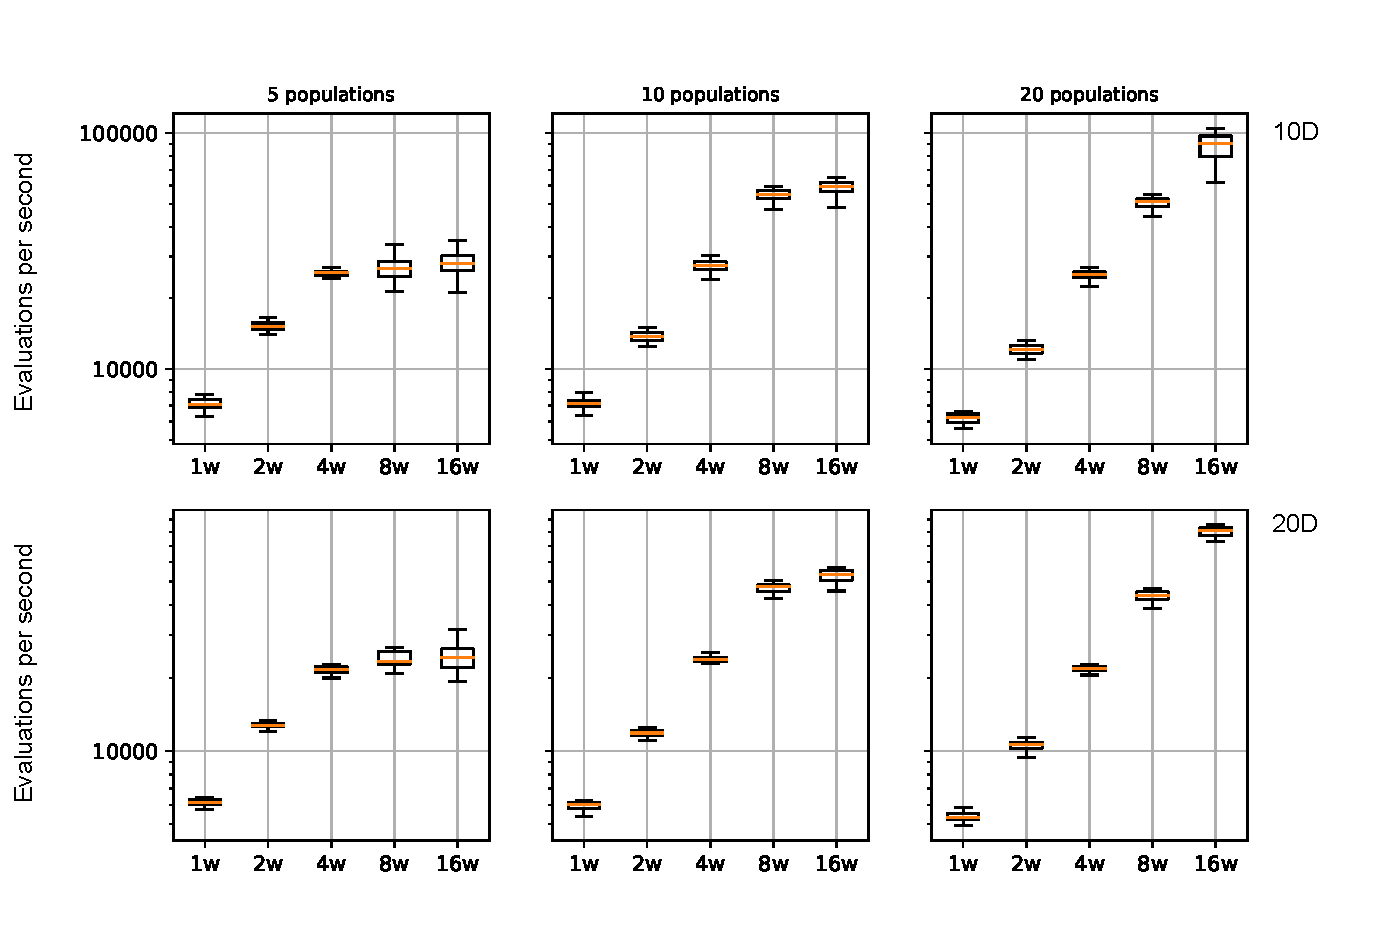
\includegraphics[width=\textwidth]{eval_ratio}
  \caption{Boxplot of the number of evaluations per second, for 30 instances of function $f_4$,
          with different number of workers and number of populations. The $y$ axis is in log scale.}
  \label{fig:spworker:evalspersecond}
\end{figure}

When comparing the results in this section, we performed the Wilcoxon Signed-Rank test, with a
significance level of 5\%. We indicate with an asterisk those results that are
not significant. % Where? - JJ

To measure the speedup obtained by the addition of workers, we will use the
number of evaluations per second, instead of the time required to finish an
instance of a problem. The reason for this is that in some cases reaching the
desired target can require less work, because we are using a stochastic search. 
We are going to measure the total increase of work done in a second by adding more workers.

\begin{table}[h!tbp]
  \caption{Speedup by worker and dimension, taking one worker as the
    baseline.}
% Clarify here what you are measuring. Number of evaluations for
% whatever divided by whatever - JJ
  \label{tab:speedup-table}
  \vspace{0.25cm}
  \centering

  \begin{tabular}{c|r|r|r|r|}
  \hline
  \multicolumn{1}{|l|}{Dimension} & \multicolumn{1}{c|}{2W} & \multicolumn{1}{c|}{4W} & \multicolumn{1}{c|}{8W} & \multicolumn{1}{c|}{16W}  \\ \hline
  \multicolumn{5}{| c|}{5 Populations} \\ \hline
  \multicolumn{1}{|c|}{10}        & \textbf{2.15} & 3.61 & 3.75 & 3.96     \\ \hline
  \multicolumn{1}{|c|}{20}        & \textbf{2.09} & 3.53 & 3.83 & 3.95     \\ \hline
  \multicolumn{5}{| c|}{10 Populations} \\ \hline
  \multicolumn{1}{|c|}{10}        & 1.91           & 3.82 & 7.67 & 8.25     \\ \hline
  \multicolumn{1}{|c|}{20}        & 1.97           & 3.97 & 7.90 & 8.90     \\ \hline
  \multicolumn{5}{| c|}{20 Populations} \\ \hline
  \multicolumn{1}{|c|}{10}        & 1.96           & \textbf{4.05} & \textbf{8.29} & \textbf{14.50}     \\ \hline
  \multicolumn{1}{|c|}{20}        & 2.00           & \textbf{4.09} & \textbf{8.18} & \textbf{15.16}     \\ \hline
  \end{tabular}
\end{table}

The baseline for the comparison will be the algorithm with a single worker, 
and the minimum amount of work available will be five populations. 
This number is selected because the controller needs at least
three populations to migrate individuals between them, and we add two more to
keep even a single worker busy all the time. Figure \ref{fig:spworker:evalspersecond} 
shows the number of function evaluations per second, achieved by a certain number of
workers, for ten and twenty dimensions of $f_4$.  


%
As expected, within the same number of populations, there is a linear speedup
when we add more workers. The speedup is marginal in those cases where there 
are fewer populations than workers.  The reason for this is that at any given time, 
there are at least two populations in the message queue, leaving some of the workers 
waiting for populations to be available in the queue.

\begin{table}[h!tbp]
  \small
  \caption{Speedup achieved with increasing the number of workers for
    each dimension showing the p-value for the Wilcoxon test. 
    Best and Worst are highlighted (bold and underlined)}
  % Say what highlights mean - JJ
  \label{tab:speedup:test}
  \vspace{0.25cm}
  \centering
  \begin{tabular}{llllll}
  Populations & Dimension  & \multicolumn{2}{l}{Increment}  & Speedup            & p-value\\
  5  & 10 & 1w & 2w  & 2.15 & 1.51E-11 \\
  & 10 & 2w & 4w  & 1.68 & 1.51E-11 \\
  & 10 & 4w & 8w  & 1.04 & 0.004942 \\
  & 10 & 8w & 16w & 1.05 & 0.072660 \\
  & 20 & 1w & 2w  & \textbf{2.09} & 1.51E-11 \\
  & 20 & 2w & 4w  & 1.69 & 1.51E-11 \\
  & 20 & 4w & 8w  & 1.08 & 5.97E-07 \\
  & 20 & 8w & 16w & {\ul 1.03} & 0.214482 \\
  &    &    &     &      &          \\
10 & 10 & 1w & 2w  & 1.91 & 1.51E-11 \\
  & 10 & 2w & 4w  & 2.00 & 1.51E-11 \\
  & 10 & 4w & 8w  & 2.01 & 1.51E-11 \\
  & 10 & 8w & 16w & 1.08 & 1.39E-05 \\
  & 20 & 1w & 2w  & 1.97 & 1.51E-11 \\
  & 20 & 2w & 4w  & 2.01 & 1.51E-11 \\
  & 20 & 4w & 8w  & 1.99 & 1.51E-11 \\
  & 20 & 8w & 16w & 1.13 & 4.24E-09 \\
  &    &    &     &      &          \\
 20 & 10 & 1w & 2w  & 1.96 & 1.51E-11 \\
  & 10 & 2w & 4w  & 2.07 & 1.51E-11 \\
  & 10 & 4w & 8w  & 2.05 & 1.51E-11 \\
  & 10 & 8w & 16w & 1.75 & 1.51E-11 \\
  & 20 & 1w & 2w  & 2.00 & 1.51E-11 \\
  & 20 & 2w & 4w  & 2.04 & 1.51E-11 \\
  & 20 & 4w & 8w  & 2.00 & 1.51E-11 \\
  & 20 & 8w & 16w & 1.85 & 1.51E-11 \\
 \end{tabular}
  \end{table}


Table~\ref{tab:speedup-table} shows the speedup obtained against the baseline of
one worker. We achieved the maximum speedup when using four workers or more with
twenty populations. On the other hand, the maximum speedup when we consider the
cost it was with eight workers. The best speedups for each number of workers are
shown in bold in the table.  



Table~\ref{tab:speedup:test} shows the speedup obtained taking as the baseline
the previous configuration, for example, when increasing from four to eight
workers, and the p-value for the Wilcoxon Signed-Rank test. There was an
increment in all cases. Again, the best effect is achieved when the number of
populations is higher than the number of workers. Configurations following this
basic rule doubled the speed or where near it. Using five populations, we
obtained the best and worst speedup depending on the number of workers (shown in
underline and bold, respectively).




\begin{figure}[h!tbp]
  \centering
  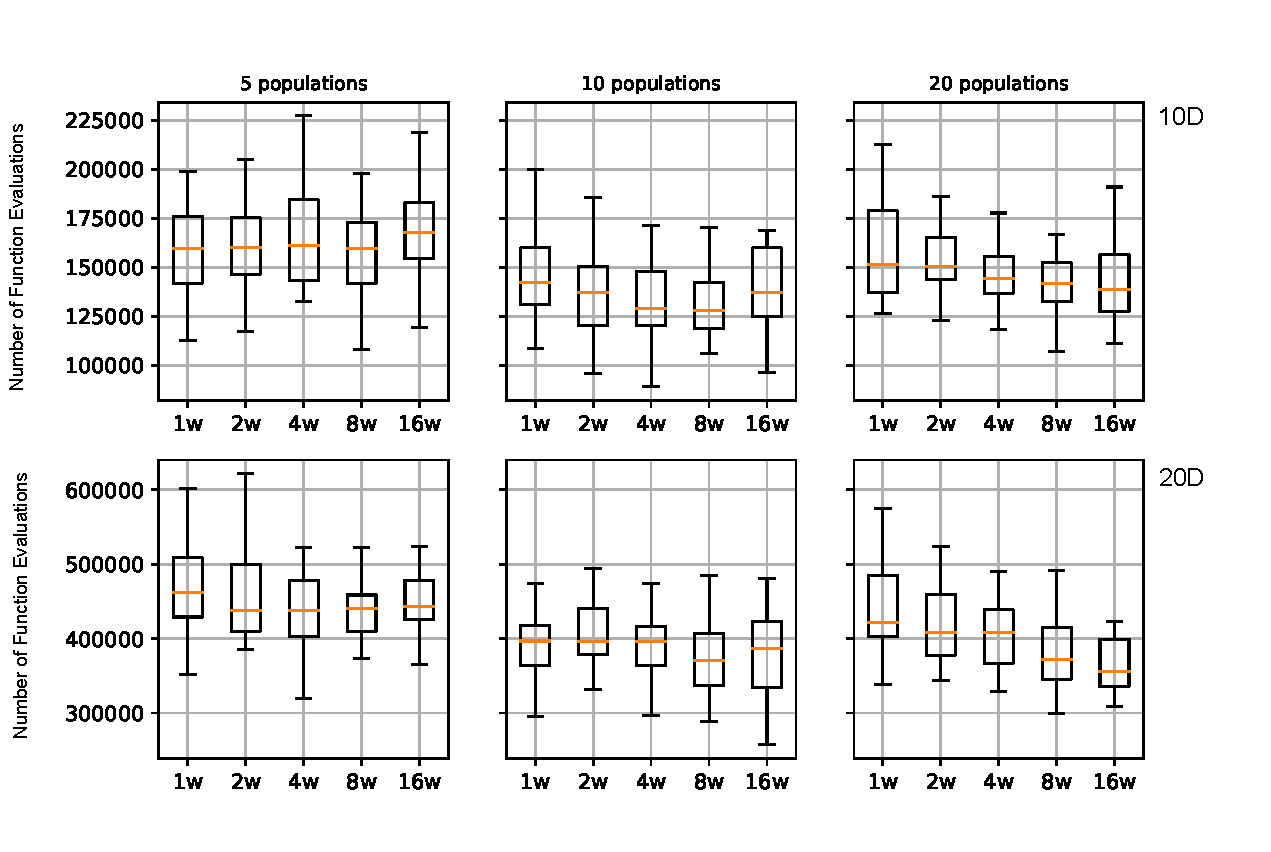
\includegraphics[width=\textwidth]{evals_per_instance}
  \caption{Boxplot of the number of function evaluations required to reach the target, for 30 instances of function $f_4$, with different number of workers and populations sizes}
  \label{fig:evals_instance}
\end{figure}




%\subsubsection{Experimental Results} 
%\label{results}

% Added some explanation % here - JJ

%We report the comparison regarding the execution time in Section~\ref{sec:exec-time}
%and the summary of the speedup in section Section~ref{sec:speedup}.
% Move this to parent - M

\subsubsection{Results Regarding Execution Time}
\label{sec:exec-time}

In the previous section, we have shown that as we increase the number of
populations and workers, we increase the ratio of the number of evaluations per
second in the same proportion. However, it is vital to notice that we can also
affect the number of evaluations we need to execute to find a solution. This
reduction means that the multi-population based algorithm can perform better
when we increase the number of populations, or in some cases, even workers, as the experiments
show. If we increase the evaluations per second and, at the same time, decrease
the number of evaluations needed, we can have a superlinear speedup of the
algorithm, if we measure the time required to complete an instance.



\begin{table}[tbp]
  \caption{Median of the number of evaluations required to finish an instance of the function $f_4$ in 30 runs
    with different number of workers and populations}
  % But this is total evaluation for all workers, right? - JJ
  \label{tab:evals_instance}
  \vspace{0.25cm}
  \centering

  \begin{tabular}{|c|c|r|r|r|}
  \hline
  \multicolumn{1}{|c}{} &   \multicolumn{1}{c}{}  & \multicolumn{3}{|c|}{Number of Populations} \\
  \hline
  Dimension           & Workers & \multicolumn{1}{c|}{5}       & \multicolumn{1}{c|}{10}      & \multicolumn{1}{c|}{20}          \\
  \hline
  \multirow{5}{*}{10} & 1w      & 159,625      & \textbf{142,368*}      & 151,680*     \\
                      & 2w      & 160,258      & \textbf{137,385}      & 150,445*     \\
                      & 4w      & 161,144      & \textbf{129,031}      & 144,354     \\
                      & 8w      & 159,893      & \textbf{{\ul 127,987}}      & 141,896     \\
                      & 16w     & 167,678      & \textbf{137,446}      & 138,852     \\
                      \hline
  \multirow{5}{*}{20} & 1w      & 462,069      & \textbf{396,841}      & 421,249*     \\
                      & 2w      & 437,952      & \textbf{395,814}      & 407,984     \\
                      & 4w      & 437,563      & \textbf{396,587}      & 408,461     \\
                      & 8w      & 440,130      & \textbf{370,264}      & 372,265     \\
                      & 16w     & 443,108      &         386,272       & \textbf{{\ul 355,999}}\\
                      \hline  
  \end{tabular}
  \end{table}


First, we will see how the configuration we selected can reduce the number of
evaluations needed in an experiment. Figure \ref{fig:evals_instance} shows the
median (30 runs) of the number of evaluations needed to complete an instance of
the function $f_4$. For every selection in the number of populations, we could
expect to have about the same number of FEs needed regardless of the number of
workers. However, we can see that for some configurations, i.e., 10D and ten
populations, eight workers will need less FEs then one (p = 0.012). Also, for
20D and twenty populations, there are differences between one and four workers
(p = 0.08) and between four and sixteen (p = 0.01). These results indicate that
there are benefits in the potential change of order in the message queue
resulting from the parallelization of work.

In Table \ref{tab:evals_instance} we can see some additional insights in more
detail. When we increase the number of populations from five to ten, or twenty,
the algorithm needs fewer FEs in both cases. The reduction is more pronounced
when using ten populations, needing fewer FEs in all but a single case (shown in
boldface). In some cases, marked with an asterisk, there is no statistical
difference between the number of evaluations; this happens when using only one
or two workers. The configurations that required less FEs have an underline in
the table.

%
\begin{figure}[h!tbp]
  \centering
  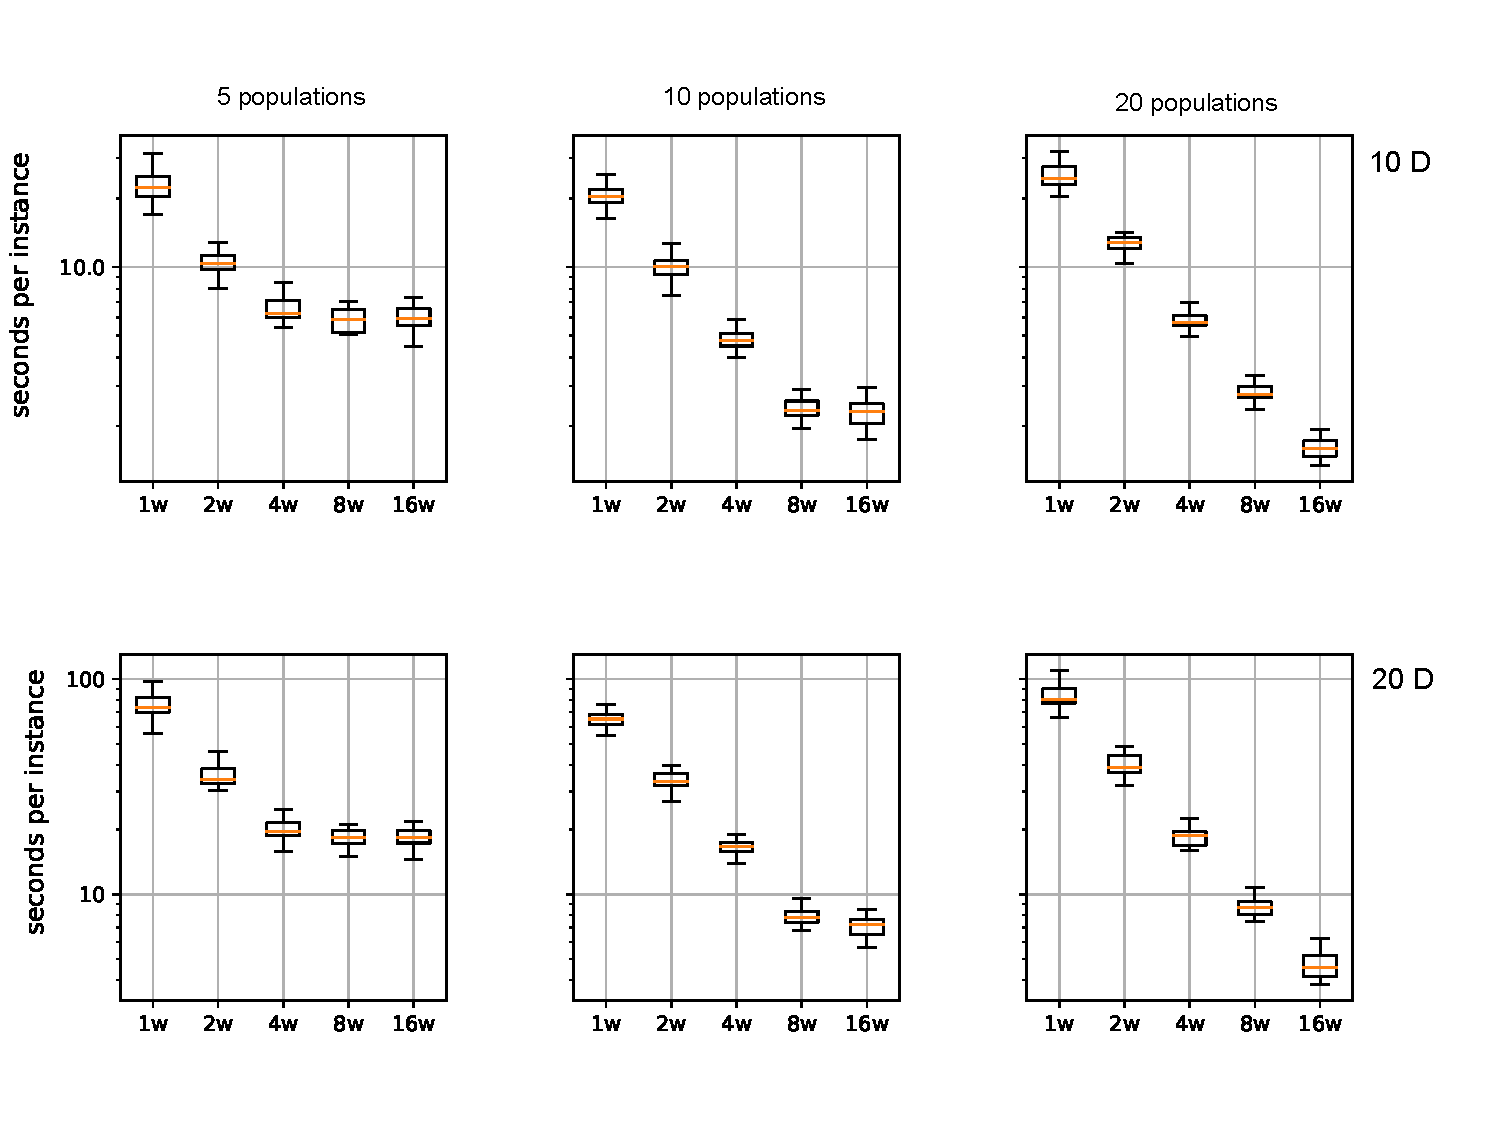
\includegraphics[width=\textwidth]{secs_per_instance}
  \caption{Boxplot of the median time required for the execution of 30 
  instances of function $f_4$, in seconds, different number of workers and 
  populations sizes. The y-axis is shown in log scale.}
  \label{fig:spworker:time}
\end{figure}
%

The reduction in the number of FEs has an impact when we measure the speed up
concerning the time needed to complete an experiment. In this case, we have
measured the median of the seconds needed to complete an instance of the
problem. Figure \ref{fig:spworker:time} shows in each box-plot the median (30
runs) of the execution time achieved by 2, 4, 8, and 16 workers, to finish an
instance of the function $f_4$, for dimensions 10 and 20, when using 5, 10, and
20 population sizes. We present each dimension in a row having a log scale on
the y-axis, to compensate for the dimension increments and scalability.  
 

\begin{table}[tbp]
  \caption{The median of the time required to finish an instance of the function $f_4$, 30 runs
  with different number of workers and populations}
  \label{tab:time}
  \vspace{0.25cm}
    \centering
    \begin{tabular}{ccrrr}
    \hline
              &         & 5 Populations    & 10 Populations & 20 Populations \\
     Dimension& Workers & Median of Time   & Median of Time & Median of Time  \\
    \hline
          10  & 1w      & 22.24  & 20.48           & 24.55  \\
              & 2w      & 10.31  & \textbf{10.00} (2.05)    & 12.79 \\
              & 4w      &  6.23  & \textbf{4.75} (2.10)     &  5.70 \\
              & 8w      &  5.86  &  \textbf{2.33} (2.03)           & 2.74 \\
              & 16w     &  5.96*  &  2.33*           & {\ul 1.59} \\
    
    \hline
          20  & 1w   & 73.87   & 65.18                 & 80.31 \\
              & 2w   & 34.18   & 33.46                 & 38.87 \\
              & 4w   & 19.55   & \textbf{16.58} (2.02) & 18.69 \\
              & 8w   & 18.38   & \textbf{7.77} (2.15)  & 8.66 \\
              & 16w  & 18.36*  & 7.27                  & {\ul 4.57} \\
    \hline
  \end{tabular}
\end{table}

In Table~\ref{tab:time} we can see that in some cases we have a supralinear
speedup, we highlighted these in boldface and indicated the speedup value in
parenthesis. The best overall times are underlined. As expected, increasing the
number of workers for a fixed dimension and populations reduced the time
required to find a solution, as long as the population number was higher than
the number of workers. The values that had no statistical difference (in the
Wilcoxon test) when increasing the number of workers have an asterisk.



\subsection{Performance of Heterogeneous Populations in the BBOB Benchmark}
\label{sec:exp2}

% Write an introduction - JJ
% I removed the Setup section, because we use the same configuration as before
% I will mention something about it - M
% mm but I don't like to have a single subsection, as I remember is not right.


\begin{figure*}[h!tb]
  \begin{tabular}
      {c@{\hspace*{-0.00001\textwidth}}
       c@{\hspace*{-0.00001\textwidth}}
       c@{\hspace*{-0.00001\textwidth}}
      }
  GA  &  PSO & GA \& PSO\\   
  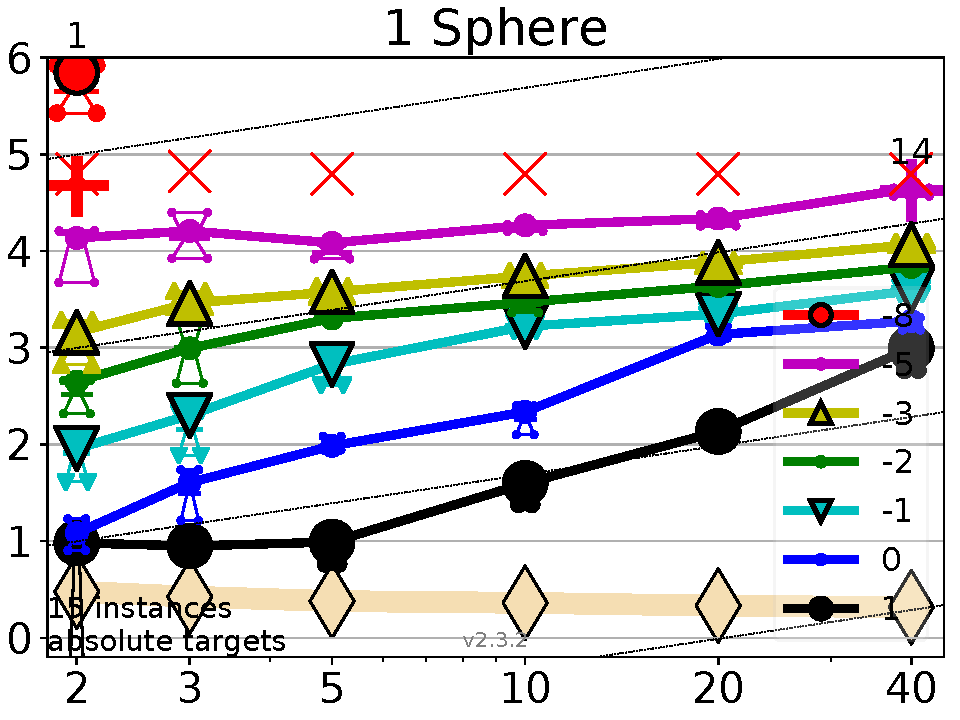
\includegraphics[width=0.30\textwidth]{GAOnly_f001}&
  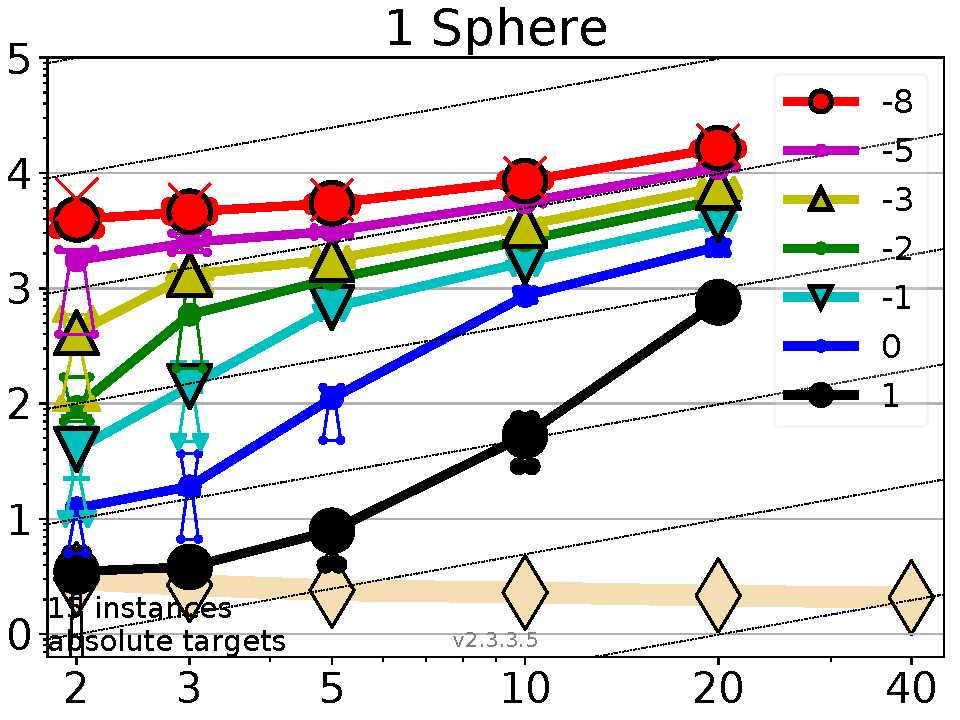
\includegraphics[width=0.30\textwidth]{PSOOnly_f001}&
  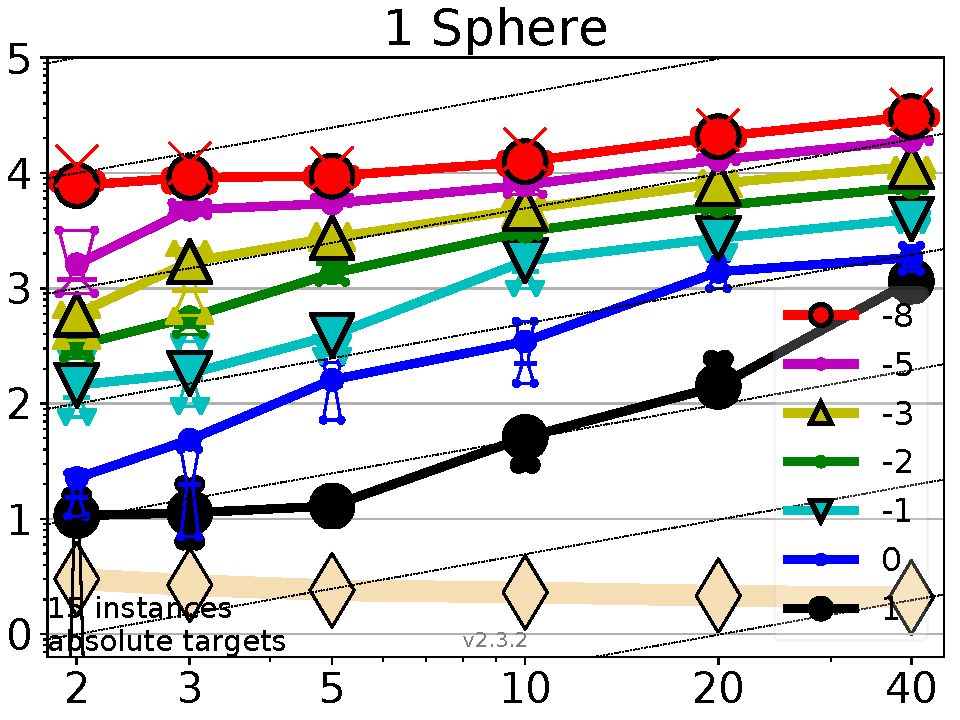
\includegraphics[width=0.30\textwidth]{GAPSO_f001}\\

  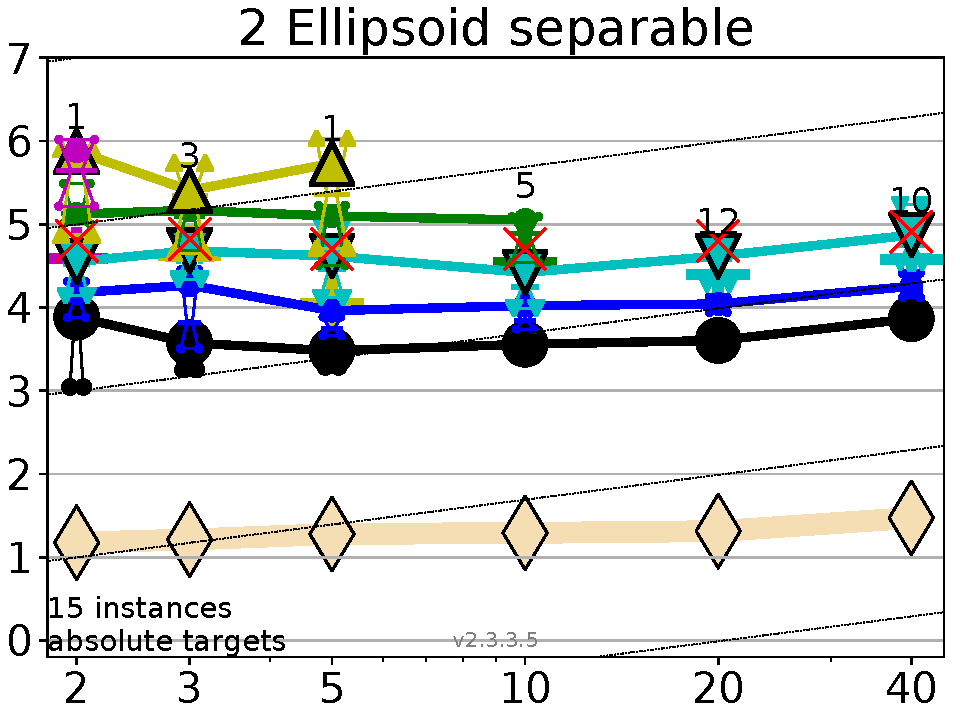
\includegraphics[width=0.30\textwidth]{GAOnly_f002}&
  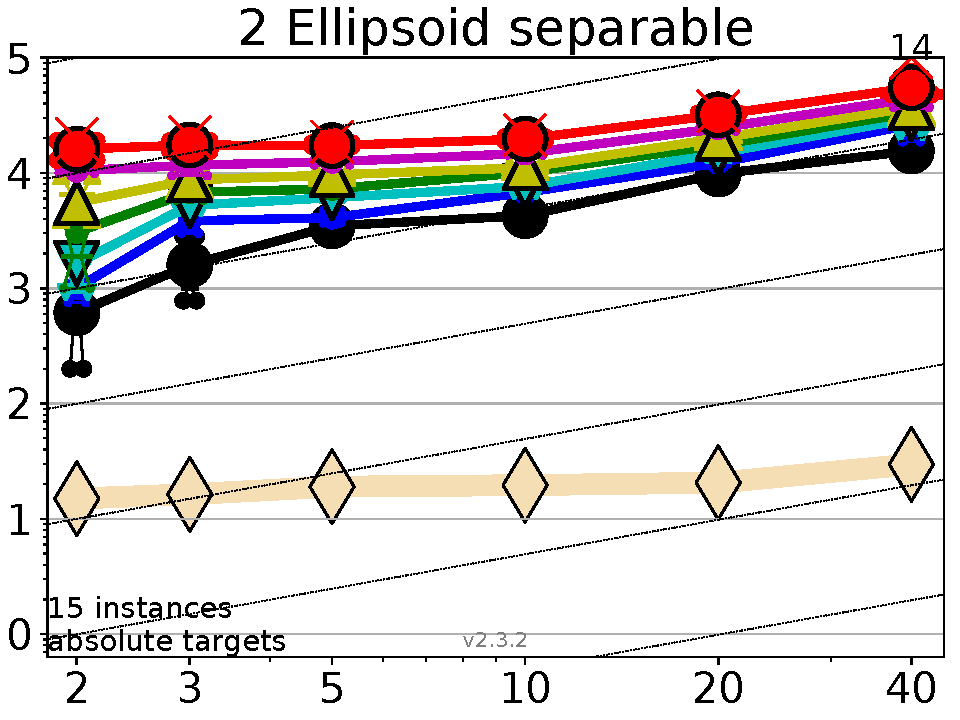
\includegraphics[width=0.30\textwidth]{PSOOnly_f002}&
  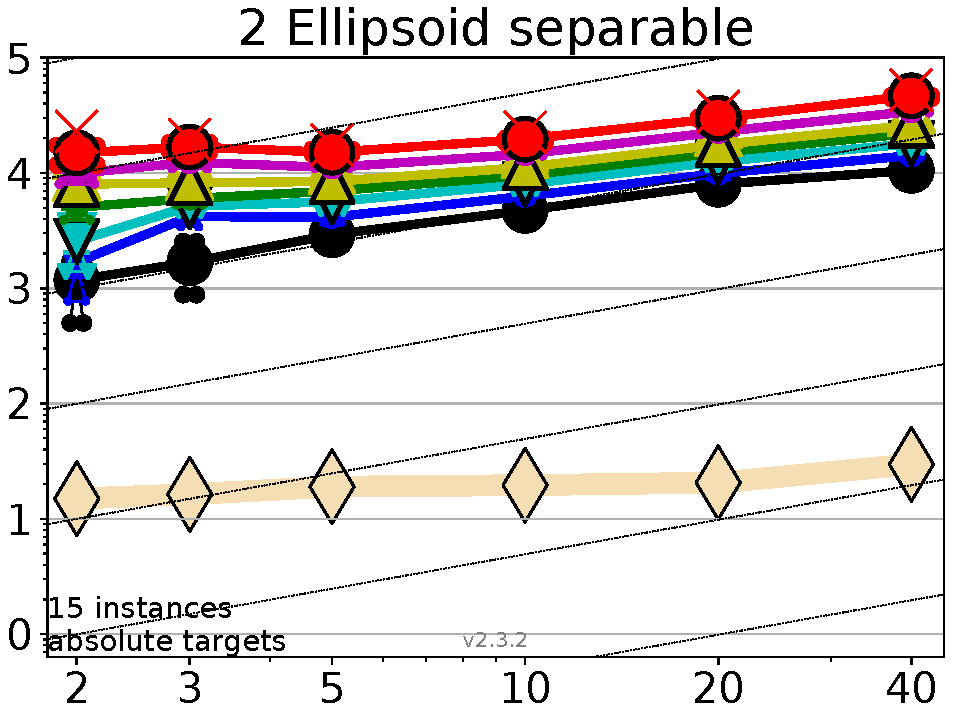
\includegraphics[width=0.30\textwidth]{GAPSO_f002}\\

  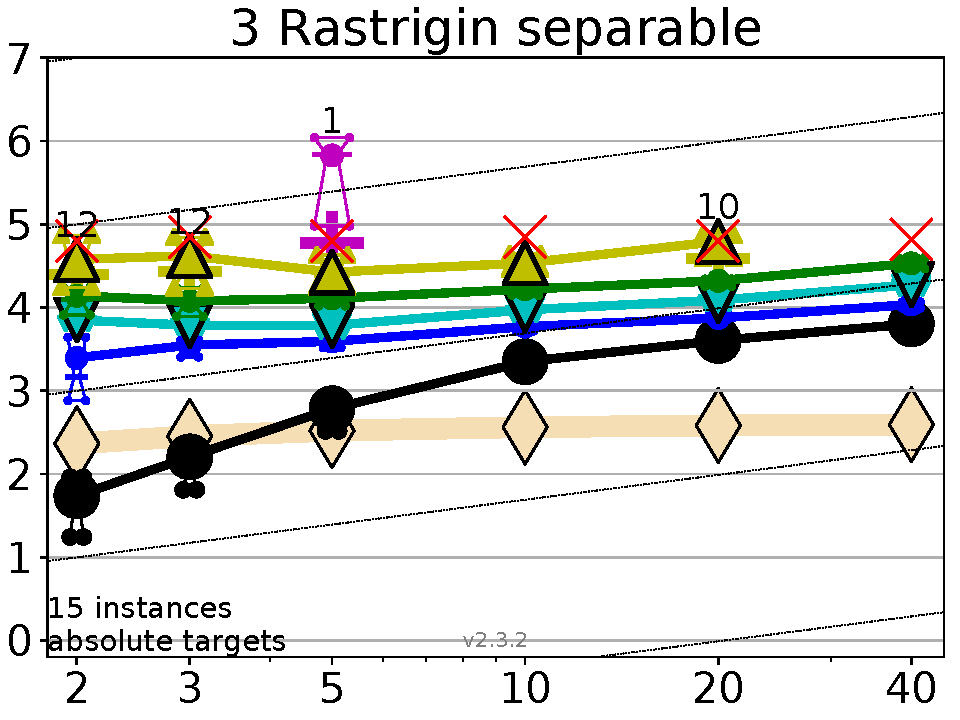
\includegraphics[width=0.30\textwidth]{GAOnly_f003}&
  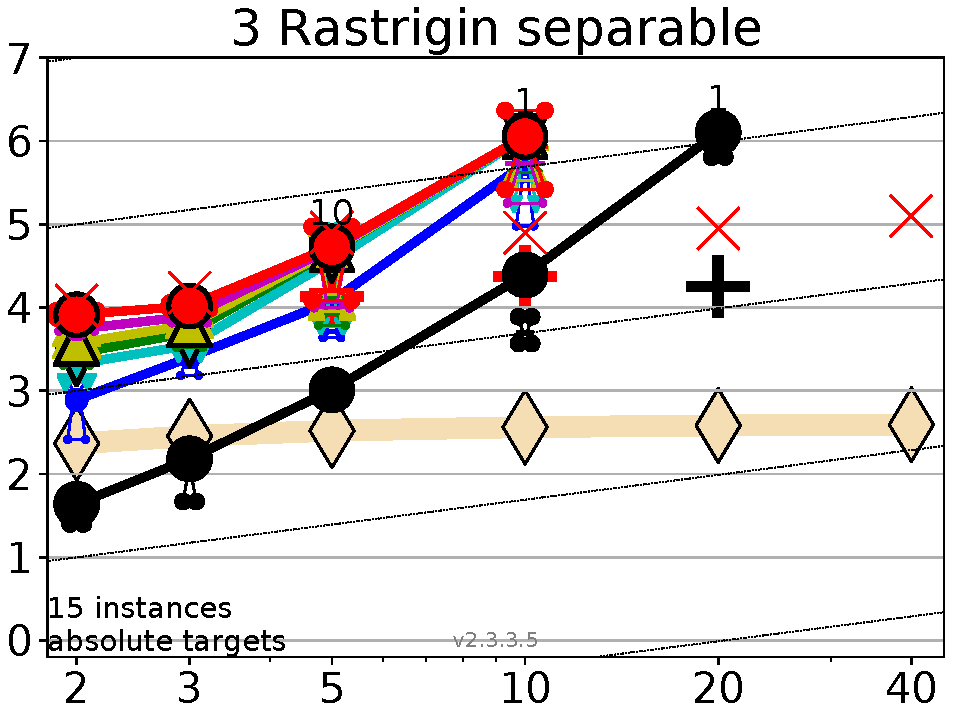
\includegraphics[width=0.30\textwidth]{PSOOnly_f003}&
  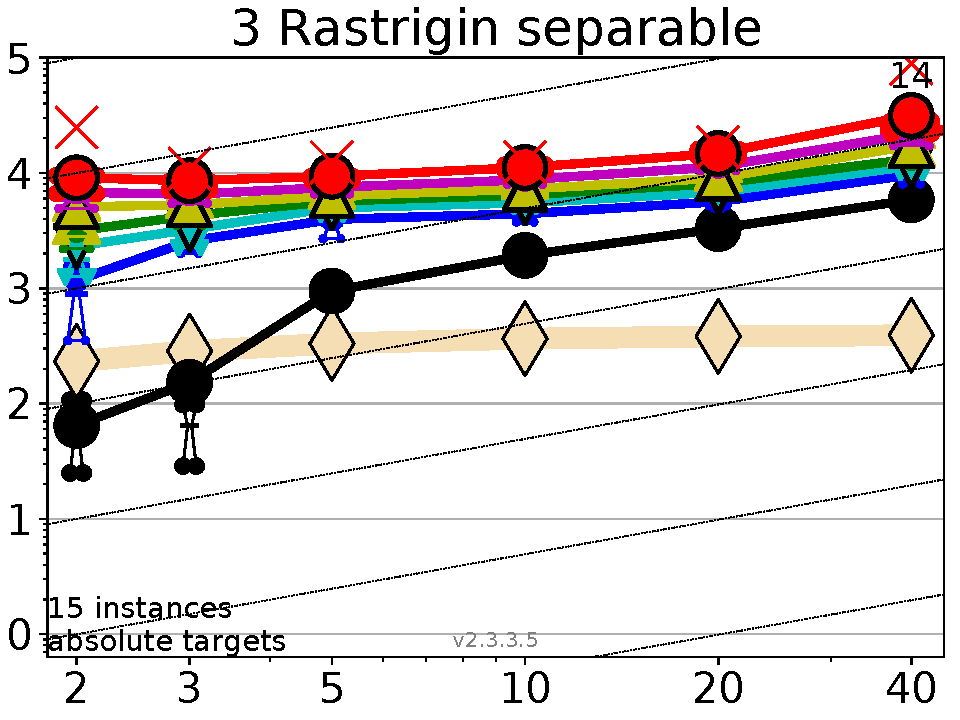
\includegraphics[width=0.30\textwidth]{GAPSO_f003}\\

  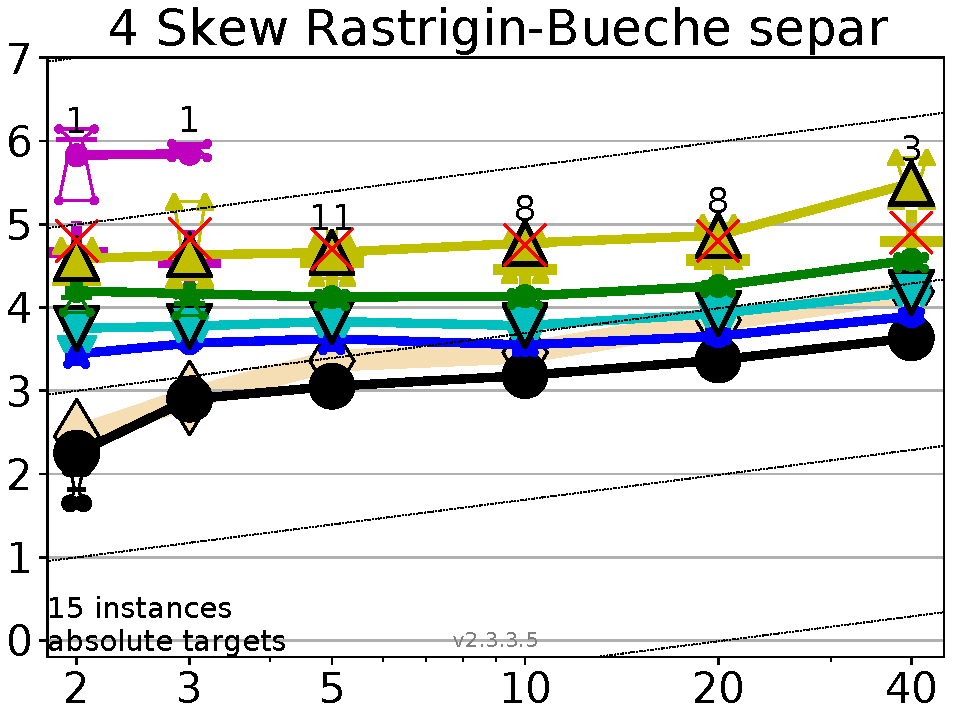
\includegraphics[width=0.30\textwidth]{GAOnly_f004}&
  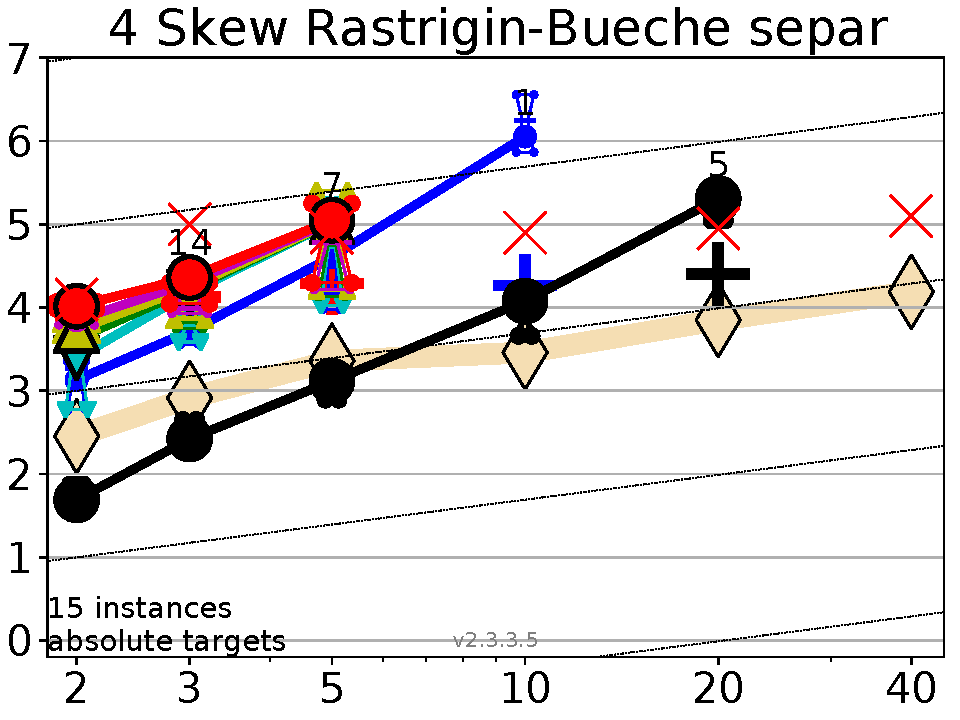
\includegraphics[width=0.30\textwidth]{PSOOnly_f004}&
  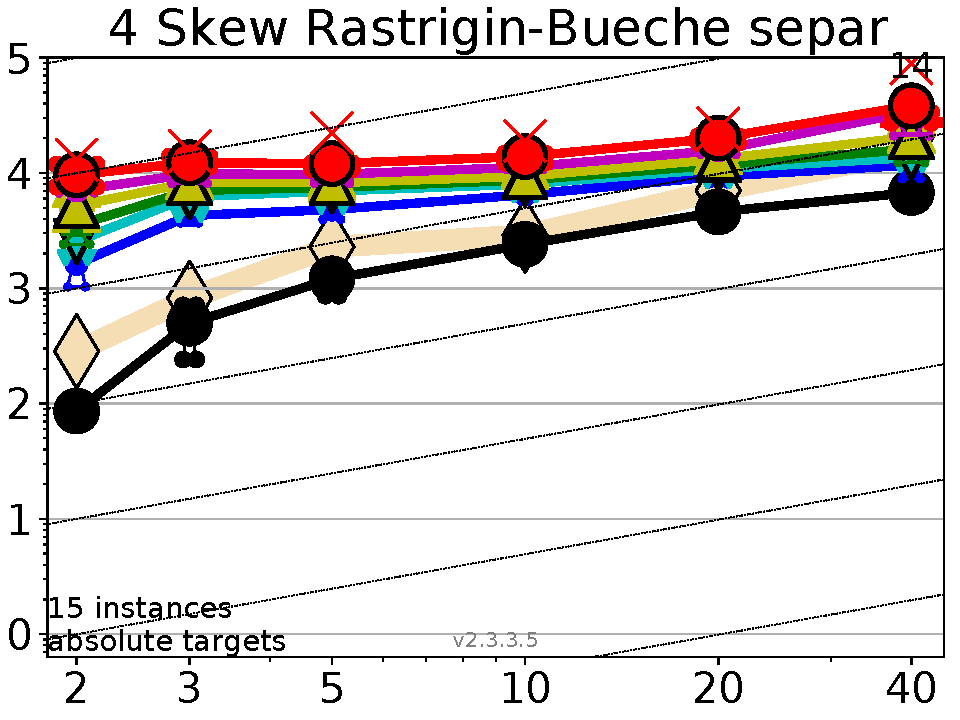
\includegraphics[width=0.30\textwidth]{GAPSO_f004}\\

  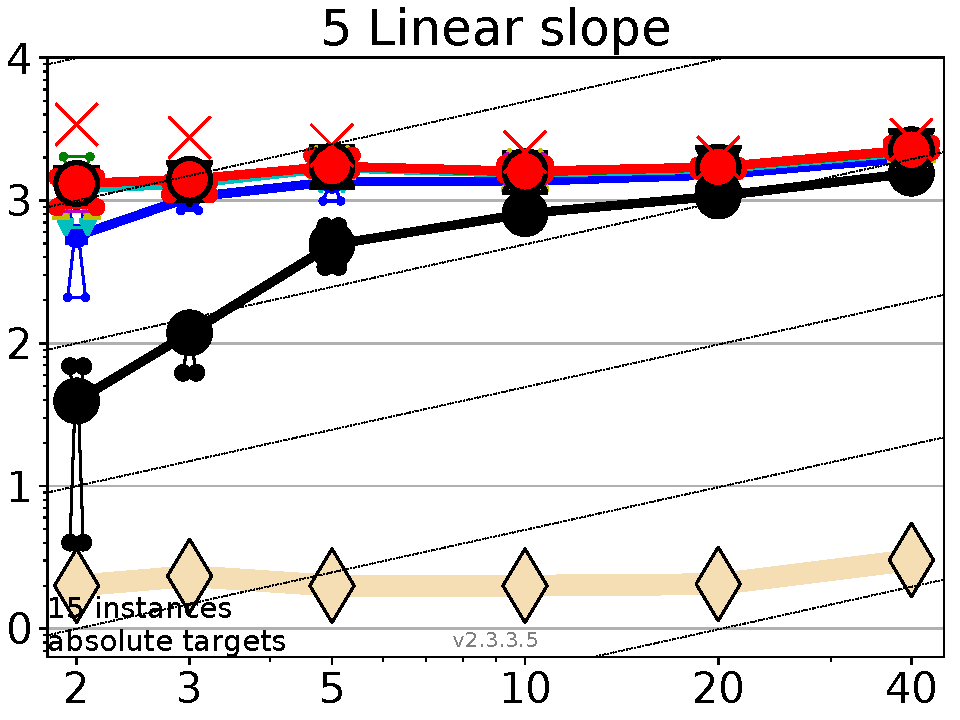
\includegraphics[width=0.30\textwidth]{GAOnly_f005}&
  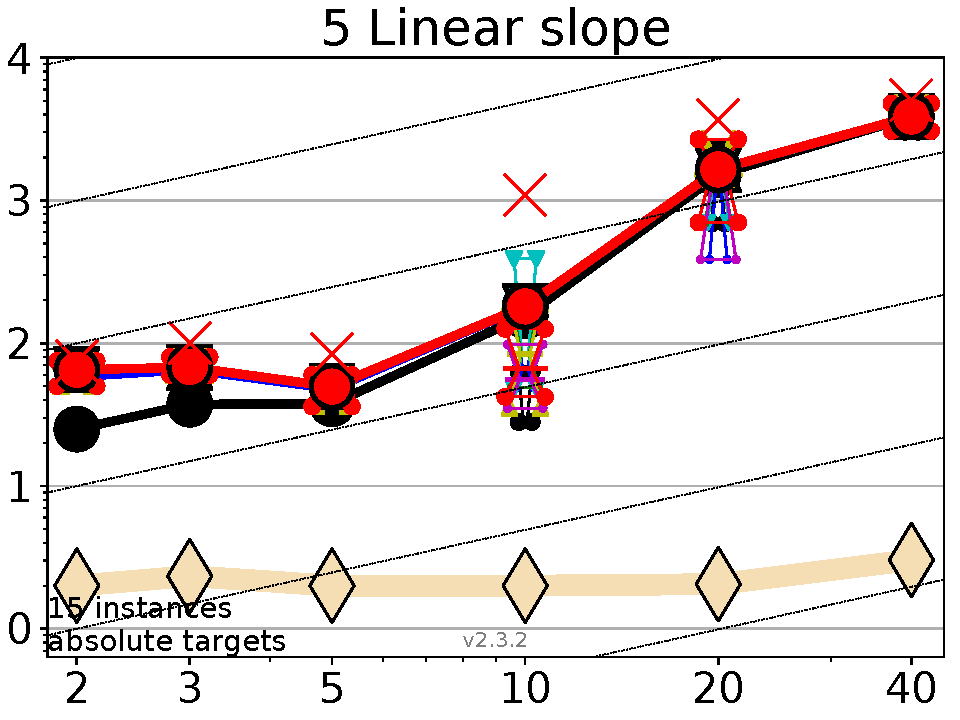
\includegraphics[width=0.30\textwidth]{PSOOnly_f005}&
  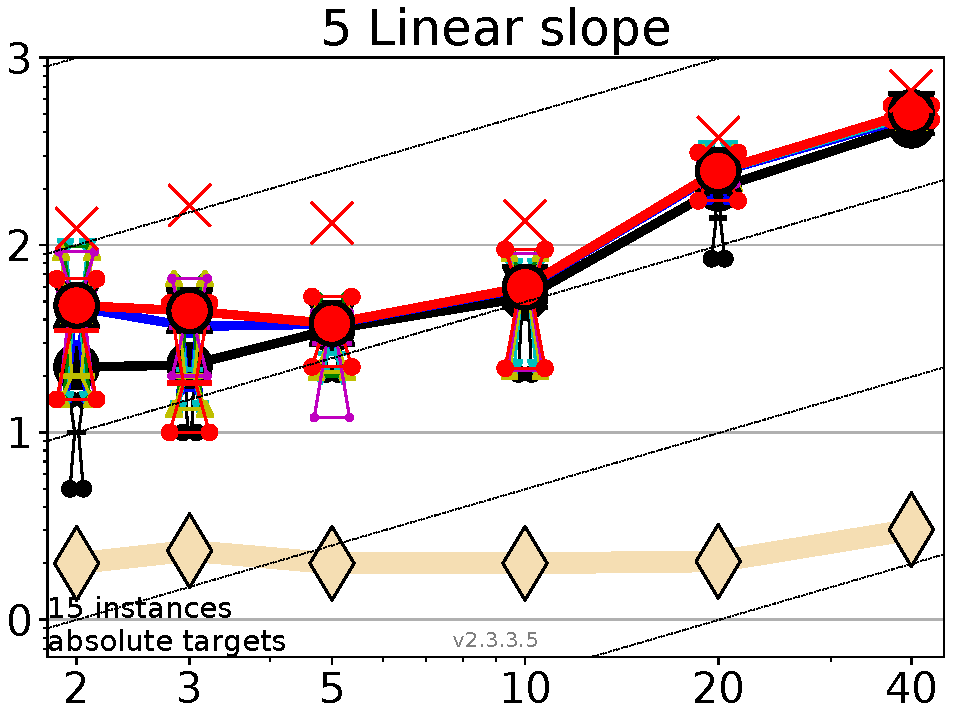
\includegraphics[width=0.30\textwidth]{GAPSO_f005}\\
  \end{tabular}
  \vspace{-3ex}
   \caption{Scaling of expected runtime (RT defined as the number of function 
evaluations \#FE) to reach a target for  
each dimension. Target values $\Delta f$ = 10, 1, $10^{-1}$, $10^{-2}$,$10^{-3}$,$10^{-5}$,$10^{-8}$
(the exponent and colors are given in the legend of $f_1$). 
Lines are the average RT; Cross ($+$): median RT of successful runs to reach
the most difficult target that was reached at least once;
Cross (\textcolor{red}{$\times$}): maximum \#FE in any trial. 
Values are divided by dimension and plotted as $log_{10}$.
The light thick line with diamonds indicates the theoretical best algorithm from BBOB 2009 for the 
most difficult target.
}
\label{fig:bbob}
\end{figure*}


%\subsubsection{Setup}

A multi-population based algorithm can decrease the execution time
thanks to running the algorithm on several populations at the same
time. But, if the populations are heterogeneous 
it might enhance evolutionary search and avoid unneeded
evaluations to a greater extent than homogeneous systems systems do; heterogeneous settings, if
done right, increase the diversity of the whole population\cite{araujo2008multikulti}.

But this is a rule of thumb, and it will depend on the degree of heterogeneity,
as well as on the algorithm itself. Some level of heterogeneity can be
implemented by just changing the configuration parameters of each population,
as in the previous experiment. But in this case, we are interested in
answering the second research question, and we want to validate if by using
heterogeneous populations and mixing search strategies,  we can increase the performance of the
search.

Therefore, in this experiment we compare a multi-population with GA and PSO only populations,
versus an ensemble of GA and PSO algorithms. We have tested on the first five functions of the
BBOB testbed; we have used ten populations and eight workers for the experiment and the
same parameters as before.

In order to run this experiment, we just needed to edit a configuration file and
start it up. The plots presented in the results are generated by the BBOB
framework from the JSON log file for each run. There was no additional setup
needed, proving how this framework is able to not only offer an reproducible way
to run experiments, but also how easily it interfaces with other common tools in
the EC ecosystem.

\subsubsection{Experimental Results} 

The results obtained by the experiments show (see Figure \ref{fig:bbob}) how
the runtime scales with dimension to reach certain target values $\Delta f$;
The color of the lines indicates the average runtime, for each target reached
at least once. A red circle without a number on top indicates the algorithm
has reached the $10^{-8}$ target on all instances for that dimension. If there
is that number, it indicates how many times the algorithm has reached
the target. Fixed values of targets $\Delta f = 10^{k}$ with $k$ colors are
given in the legend of $f_1$ in the top row, $k$ values are $[-8,-5,-3,-2,-1,0,1]$. Results
from each configuration are presented in each column, GA, PSO, and GA\&PSO
populations. 

We can see that the GA algorithm (on the leftmost column) has a hard time reaching even the
$10^{-5}$ target in functions ($f_1-f_4$) for all dimensions, and has the worst
performance in 20 and 40 dimensions. Finally, it performs better on $f_5$
reaching the $10^{-8}$ on all dimensions but with a higher runtime on lower
dimensions.

On the other hand, the multi-population PSO (taking the column on the middle) 
has better performance; its results are spread over a smaller range,
reaching all targets for functions $f_1$ and $f_2$ but with a slightly higher
runtime than the multi-strategy configuration. It is not able to reach the
$10^{-8}$ target on the higher dimensions of $f_3$ and $f_4$. Moreover, the PSO
multi-population has the best runtime for the lower dimensions of $f_5$.

Finally, the proposed PSO\&GA mixed algorithm has reached the $10^{-8}$ target
value on all functions ($f_1-f_5$) and scales well to higher dimensions, even on
$f_3$ and $f_4$ (charts on the lower rows), which are usually considered
difficult functions. This experiment also exemplifies the type of analyses that
we can perform with the results of the EvoSwarm application by reusing the COCO framework.
We also proved that multi-population algorithms can be compared under the same 
conditions, including single and multi-algorithm versions, and results show 
that the later have better performance.


\section{Conclusions} 
\label{conclusions}

In this paper we have presented the EvoSwarm framework for 
the reproducible execution of experiments with an event-based, cloud-native architecture 
suitable for hosting multi-population, multi-algorithm optimization
methods. 
The framework is based in industry-standard development
tools such as Docker and Docker Compose, making it easy for scientists and practitioners to develop and deploy
% The last version still uses Docker Compose? - JJ
multi-algorithm distributed experiments. The model implemented by the
framework is based on the asynchronous
exchange of messages between stateless functions that react to a continuous
stream of data; populations are the messages that flow in this stream. We show the differences of the message-driven architecture we presented against
four other proposals for multi-population algorithms found in the literature, and highlight the 
advantages for conducting asynchronous multi-population algorithms.

We have proposed a new methodology for the reproducible deployment and execution of
multiple experiments by specifying the infrastructure as part of an experiment
definition in both local and cloud environments. We presented the workflow of an
experiment's entire life-cycle viewed from the perspective of developers and
researchers. 
We have tested the deployment of an experiment on Amazon's Elastic
Container Service, and proved that as a cloud-native, container-based application,
EvoSwarm could be deployed locally or in the cloud by specifying the configuration 
of container images and resources in an orchestration service.

We have performed an empirical evaluation of the same framework to learn if the proposed
solution can efficiently improve the scalability and performance of
population-based optimization algorithms.

First, we focused on knowing how scaling is related to the number of populations
and workers in the system. This experiment concludes that there is an
interesting interplay between them, with the most benefit obtained with a number of
populations slightly above the number of workers, which brings performance gains 
in terms of execution speed; these experiments take less time since
evaluations are performed, as part of its corresponding algorithm, simultaneously by different workers.
Also, we found that for lower dimensions, there is an advantage in using fewer
populations. % Specify that.

A second experiment centered on evaluating the algorithmic benefits (experiments
taking less time because they need fewer evaluations) of distributed
multi-algorithm algorithms such as the ones implemented in this kind of framework.
We compared the homogeneous and an ensemble of
multi-populations, using Genetic Algorithms (GAs) and Particle Swarm
Optimization (PSO) using the COCO benchmark framework 
for visualization and definition of the optimization problems.
We found that the set-up of these algorithms has a significant influence on
their results since diversity is essential for their performance. The
hybrid method using both algorithms 
achieved better results and, in most cases, needed fewer evaluations. % Clarify if they actually achieve that way superlinear improvements - JJ

% Probably a final conclusion should be added here - JJ<

This work also opens new possibilities. From the design point of view, it would
be interesting to use automatic scaling, instead of setting the number of
workers by hand. This would need a certain amount of configuration, as we would
be using container orchestration with auto-scaling capabilities such as
Kubernetes or Docker Swarm. The current orchestration (Amazon ECS) also has
auto-scaling capabilities, but additional configuration is needed; also, we need
to establish the auto-scaling of both containers and Amazons EC2 instances.
Instead of setting a fixed number of workers, only the maximum amount would need
to be established, which could be done directly or by setting an evaluation
budget.

From the algorithmic point of view, there are many possible lines of
research. Mixing population-based algorithms with other algorithms
would be a possibility, but also using different instances of
population based algorithms, such as checking how Estimation of
Distribution Algorithms would work together with evolutionary
algorithms. EvoloPy also includes other population based algorithms,
which could be tested, trying to find out which sets of algorithms are
a better match to each other. All these will be explored as future
lines of work.

\section{Acknowledgements}

This paper has been supported in part by projects TecNM-5654.19-P and DeepBio
(TIN2017-85727-C4-2-P).

%\section*{References}

\bibliographystyle{elsarticle-num}
\bibliography{multipopulation}

\end{document}